% =====================================================================
%  Tesina (versión reducida) — Impacto de shocks informativos en el
%  comportamiento bursátil de empresas argentinas
%  Gino Frigoni · Nicolás Diddi
%
%  Mismo formato que Tesina_Final.tex (la versión completa, que no se modifica).
%  Foco: los cuatro instrumentos (corpus, FinBETO, VIX argentino, HMM) y el
%  experimento que los usa (VAR y Granger).
%  Compilar desde esta carpeta:  python compilar_reducida.py
% =====================================================================
\documentclass[11pt,a4paper,oneside]{report}

% ---------- Idioma y fuentes ----------
\usepackage{fontspec}
\setmainfont{Georgia}
\setsansfont{Arial}
\setmonofont{Consolas}[Scale=0.88]
\newfontfamily\titulos{Arial}
\usepackage[spanish,es-tabla,es-noshorthands]{babel}
\usepackage[autostyle]{csquotes}
\usepackage{microtype}

% ---------- Página ----------
\usepackage[left=3cm,right=2.5cm,top=2.8cm,bottom=2.6cm,headheight=15pt]{geometry}
\usepackage{setspace}
\setstretch{1.18}
\setlength{\parindent}{0pt}
\setlength{\parskip}{0.55em}

% ---------- Paquetes ----------
\usepackage[table]{xcolor}
\usepackage{graphicx}
\graphicspath{{figuras/}{./}}
\usepackage{booktabs}
\usepackage{tabularx}
\usepackage{longtable}
\usepackage{array}
\usepackage{multirow}
\usepackage{enumitem}
\usepackage{fancyhdr}
\usepackage{titlesec}
\usepackage{amsmath}
\usepackage{amssymb}
\usepackage{caption}
\usepackage{float}
\usepackage{lastpage}
\usepackage[round]{natbib}
\setcitestyle{aysep={,},yysep={;}}
\usepackage[obeyspaces,spaces]{url}
\usepackage[hidelinks,bookmarksnumbered,bookmarksopen,pdfusetitle]{hyperref}
\hypersetup{pdftitle={Impacto de shocks informativos en el comportamiento bursátil de empresas argentinas},
            pdfauthor={Gino Frigoni; Nicolás Diddi}}

% ---------- Colores ----------
\definecolor{gris}{HTML}{5B6472}
\definecolor{acento}{HTML}{1F4E79}
\definecolor{celda}{HTML}{DCE6F0}
\definecolor{plan}{HTML}{C9D3DE}
\definecolor{real}{HTML}{1F4E79}

% ---------- Títulos (Arial, como el modelo) ----------
\titleformat{\chapter}[display]
  {\titulos\bfseries\color{acento}}
  {\large\chaptertitlename\ \thechapter}{4pt}
  {\LARGE}[\vspace{2pt}{\color{gris}\titlerule[0.5pt]}]
\titlespacing*{\chapter}{0pt}{0pt}{22pt}
\titleformat{\section}{\titulos\large\bfseries}{\thesection}{0.7em}{}
\titleformat{\subsection}{\titulos\normalsize\bfseries}{\thesubsection}{0.7em}{}
\titleformat{\subsubsection}{\titulos\normalsize\itshape}{}{0em}{}
\titlespacing*{\section}{0pt}{18pt}{6pt}
\titlespacing*{\subsection}{0pt}{14pt}{4pt}
\titlespacing*{\subsubsection}{0pt}{10pt}{2pt}
\setcounter{secnumdepth}{2}
\setcounter{tocdepth}{2}

% ---------- Encabezado y pie (como el modelo) ----------
\newcommand{\titulocorto}{Impacto de shocks informativos en el comportamiento bursátil de empresas argentinas}
\pagestyle{fancy}
\fancyhf{}
\fancyhead[C]{\titulos\footnotesize\itshape\color{gris}\titulocorto}
\fancyfoot[L]{\titulos\footnotesize Autores: Gino Frigoni + Nicolás Diddi}
\fancyfoot[R]{\titulos\footnotesize Pág. \thepage\ de \pageref*{LastPage}}
\renewcommand{\headrulewidth}{0.4pt}
\fancypagestyle{plain}{\fancyhf{}%
  \fancyhead[C]{\titulos\footnotesize\itshape\color{gris}\titulocorto}%
  \fancyfoot[L]{\titulos\footnotesize Autores: Gino Frigoni + Nicolás Diddi}%
  \fancyfoot[R]{\titulos\footnotesize Pág. \thepage\ de \pageref*{LastPage}}}

% ---------- Epígrafes: debajo, con la fuente ----------
\captionsetup{font=small,labelfont=bf,labelsep=period,justification=justified,singlelinecheck=true}
\captionsetup[table]{position=below,skip=6pt}
\captionsetup[figure]{skip=6pt}
\renewcommand{\arraystretch}{1.2}
\setlength{\tabcolsep}{4.5pt}
\setlength{\emergencystretch}{2.5em}

% ---------- Listas ----------
\setlist{itemsep=2pt,topsep=3pt,parsep=0pt}

% ---------- Bibliografía ----------
\renewcommand{\bibname}{Bibliografía}
\setlength{\bibsep}{5pt plus 1pt}
\renewcommand{\bibfont}{\small}
\renewcommand{\UrlFont}{\ttfamily\small}
% Las rutas y los nombres de variables pueden cortarse también en los guiones bajos.
\makeatletter\g@addto@macro{\UrlBreaks}{\do\_}\makeatother

% ---------- Atajos ----------
% Archivo de un paper o carpeta del proyecto, relativo a la carpeta raíz de la tesis;
% el enlace abre el archivo desde el PDF (lectores de PDF de escritorio).
\newcommand{\archivo}[1]{\href{run:../#1}{\nolinkurl{#1}}}
\newcommand{\carpeta}[1]{\nolinkurl{#1}}
\newcommand{\var}[1]{\texttt{#1}}
\newcommand{\flecha}{$\rightarrow$}
\newcommand{\fuente}[1]{\par\vspace{2pt}{\footnotesize\textit{Fuente:} #1\par}}
% Datos que completan los autores antes de entregar
\newcommand{\completar}[1]{\textcolor{red!70!black}{[#1]}}
\newcolumntype{L}[1]{>{\raggedright\arraybackslash}p{#1}}
\newcolumntype{C}[1]{>{\centering\arraybackslash}p{#1}}
\newcolumntype{Y}{>{\raggedright\arraybackslash}X}

% Recuadro con fondo, para notas al margen del texto principal (p. ej., el NER)
\newenvironment{recuadro}[1]
  {\par\vspace{4pt}\noindent\begin{lrbox}{\recuadrobox}\begin{minipage}{\dimexpr\linewidth-2\fboxsep-2\fboxrule\relax}
   \setlength{\parskip}{0.45em}\small{\titulos\bfseries\color{acento}#1}\par}
  {\end{minipage}\end{lrbox}\fcolorbox{acento}{celda!45}{\usebox{\recuadrobox}}\par\vspace{4pt}}
\newsavebox{\recuadrobox}

\begin{document}

% =====================================================================
%  PORTADA
% =====================================================================
\begin{titlepage}
  \titulos
  \begin{center}
    
\includegraphics[width=6cm]{logo_ugr.png}\par
    \vspace{0.8cm}
    {\large\bfseries TRABAJO FINAL DE GRADO\par}
    \vspace{0.3cm}
    {\normalsize Presentado para lograr el título de\par}
    \vspace{0.2cm}
    {\large\bfseries LICENCIADO EN CIENCIA DE DATOS\par}
    \vspace{0.2cm}
    {\normalsize Seminario de Trabajo Final\par}
    \vspace{1.6cm}
    {\color{gris}\rule{\linewidth}{0.6pt}}\par
    \vspace{0.6cm}
    {\LARGE\bfseries «Impacto de shocks informativos en el comportamiento bursátil de
    empresas argentinas: un enfoque basado en análisis de sentimiento y modelos de series
    temporales»\par}
    \vspace{0.6cm}
    {\color{gris}\rule{\linewidth}{0.6pt}}\par
    \vfill
    {\large Autores\par}
    \vspace{0.3cm}
    \begin{tabular}{l@{\qquad}l}
      Gino Frigoni   & DNI 31.356.373 \\[2pt]
      Nicolás Diego Diddi & DNI 46.443.733 \\
    \end{tabular}
    \vspace{1.4cm}

    {\large Rosario, \rule{4.5cm}{0.4pt}\par}
    \vspace{1.6cm}
    \begin{tabular}{c@{\hspace{2.5cm}}c}
      \rule{5cm}{0.4pt} & \rule{5cm}{0.4pt} \\
      Firma autor & Firma autor \\
    \end{tabular}
  \end{center}
\end{titlepage}
\setcounter{page}{2}  % la portada cuenta como página 1, como en el modelo

% =====================================================================
%  RESUMEN
% =====================================================================
\chapter*{Resumen}
\addcontentsline{toc}{chapter}{Resumen}
\begin{center}
  {\titulos\large\bfseries Impacto de shocks informativos en el comportamiento bursátil de
  empresas argentinas: un enfoque basado en análisis de sentimiento y modelos de series
  temporales\par}
\end{center}
\vspace{4pt}

Este trabajo estudió si las noticias económicas publicadas por los medios digitales
argentinos anticipan el precio y el volumen operado de las acciones que cotizan en Bolsas y
Mercados Argentinos (BYMA). Para responderlo hubo que construir cuatro instrumentos que no
existían para el mercado argentino. Del lado de las noticias, un corpus de 14.012 notas de
siete portales, recolectado con la Wayback Machine y los mapas del sitio y depurado de
duplicados, plantillas y contenido que no era noticia; y FinBETO, un modelo BETO adaptado a la
prensa económica y ajustado para clasificar oraciones en cuatro clases, que funciona como un
termómetro del tono de las noticias (F1 macro de 0,685 en noticias no vistas, contra 0,546 del
modelo de referencia en tres clases). Del lado del mercado, un VIX argentino construido con la
volatilidad realizada del S\&P~Merval, que reacciona con claridad a la salida del cepo y a las
dos elecciones de 2025; y un modelo oculto de Markov que divide el período en tres regímenes
(Calmo, Moderado y Tenso). Los cuatro instrumentos se unieron en 244 ruedas, de mayo de 2025 a
abril de 2026, y se contrastaron con modelos VAR y pruebas de causalidad de Granger. El tono de
las noticias no anticipó los precios ni el volumen, en ningún nivel ni régimen. Apareció, en
cambio, la relación inversa: el retorno del S\&P~Merval anticipa el tono de las notas
siguientes, en 39 de las 47 empresas y en 15 de las 17 con tono propio, con el efecto
concentrado en las notas publicadas la misma noche, después del cierre. Los medios económicos
argentinos, en el período estudiado, siguieron al mercado.

\vspace{6pt}
\textit{Palabras clave:} \textit{web scraping; análisis de sentimiento; BETO; volatilidad
realizada; modelos ocultos de Markov; causalidad de Granger; S\&P~Merval.}

\textit{Temática de Interés en Ciencia de Datos:} \textit{procesamiento de lenguaje natural
y econometría de series de tiempo aplicados a mercados financieros.}

% =====================================================================
%  ÍNDICE
% =====================================================================
\tableofcontents

% =====================================================================
%  GLOSARIO
% =====================================================================
\chapter*{Siglas y términos}
\addcontentsline{toc}{chapter}{Siglas y términos}
\begin{longtable}{@{}L{2.6cm}L{11.3cm}@{}}
\toprule
\textbf{Sigla} & \textbf{Significado} \\
\midrule
\endhead
ADF & Prueba de Dickey-Fuller aumentada (raíz unitaria). \\
AIC / BIC & Criterios de información de Akaike y bayesiano (Schwarz). \\
BETO & Modelo BERT preentrenado en español (Universidad de Chile). \\
BH & Corrección de Benjamini-Hochberg por pruebas múltiples. \\
BYMA & Bolsas y Mercados Argentinos. \\
CAR & Retorno anormal acumulado (\textit{cumulative abnormal return}). \\
CCL & Dólar contado con liquidación. \\
CRISP-DM & Proceso estándar para proyectos de minería de datos. \\
DLM & Modelo de rezagos distribuidos (\textit{distributed lag model}). \\
EWMA & Media móvil con ponderación exponencial. \\
F1 macro & Promedio simple del F1 de cada clase. \\
FinBETO & BETO adaptado al dominio de la prensa económica y ajustado para sentimiento. \\
HMM & Modelo oculto de Markov; aquí, modelo de cambio de régimen de Markov. \\
IRF & Función de impulso-respuesta. \\
KPSS & Prueba de estacionariedad de Kwiatkowski, Phillips, Schmidt y Shin. \\
MLM & Modelado de lenguaje enmascarado (\textit{masked language modeling}). \\
MST & Árbol de expansión mínima (\textit{minimum spanning tree}). \\
NER & Reconocimiento de entidades nombradas. \\
OLS / MCO & Mínimos cuadrados ordinarios. \\
Rueda & Día hábil de operación en BYMA (de 11:00 a 17:00). \\
Tono & Sentimiento neto: \% de oraciones positivas menos \% de negativas. \\
Tono anormal & Tono de la rueda menos el promedio de las 20 ruedas previas. \\
Tono propio & Cuánto mejor o peor se habla de una empresa que del mercado, ponderado por la cantidad de oraciones. \\
VAR & Vector autorregresivo. \\
VIX argentino & Volatilidad realizada del S\&P~Merval en 20 ruedas, anualizada. \\
\bottomrule
\end{longtable}

% =====================================================================
%  CUERPO
% =====================================================================
% =====================================================================
\chapter{Introducción}
\label{cap:introduccion}

Los mercados financieros se mueven con la información. Un dato de inflación, un anuncio del
Banco Central o el resultado de una elección cambian lo que los inversores esperan de las
empresas, y esas expectativas se trasladan a los precios y al volumen operado. Los medios
económicos son uno de los canales por los que esa información circula. Desde hace casi dos
décadas, la literatura financiera estudia si el tono de esas notas ayuda a anticipar el
comportamiento de las acciones o si se limita a contar lo que el mercado ya hizo
\citep{tetlock2007,garcia2013,verma2026}.

% ---------------------------------------------------------------------
\section{Problemática observada}

En la conversación cotidiana sobre la bolsa argentina está muy extendida la idea de que «las
noticias mueven las acciones». La observación tiene sustento intuitivo, porque los días de
noticias grandes, como los posteriores a una elección, son también días de movimientos fuertes
del S\&P~Merval. Pero esa coincidencia no dice qué vino primero: es posible que las noticias
muevan al mercado, y también que los medios cuenten lo que el mercado ya hizo. El problema de
este trabajo es separar esas dos posibilidades con datos, ordenando en el tiempo el tono y la
cantidad de las noticias económicas y el precio y el volumen de las acciones. Para el mercado
argentino no había con qué responderlo: ni un corpus de prensa económica, ni un modelo de
sentimiento entrenado para ese lenguaje, ni un índice de volatilidad como el VIX de Chicago, ni
una clasificación de los días según el estado del mercado.

% ---------------------------------------------------------------------
\section{Hipótesis de investigación}

El plan de trabajo define el \textit{shock informativo} como un aumento anormal del volumen
de noticias publicadas por medios digitales argentinos sobre temas económico-financieros, y
plantea las siguientes hipótesis:

\begin{quote}
\textbf{Hipótesis alternativa (H1).} «El shock informacional tiene un impacto medible y
estadísticamente significativo sobre el comportamiento bursátil —precio y/o volumen de
transacciones— de las empresas argentinas que cotizan en bolsa.»

\textbf{Hipótesis nula (H0).} «El shock informacional no tiene un impacto estadísticamente
significativo sobre el comportamiento bursátil de las empresas argentinas.»
\end{quote}

El shock se midió de dos maneras complementarias: por su \textit{tono} (ruedas en que las
noticias son mucho más positivas o negativas que lo habitual) y por su \textit{cantidad}
(ruedas con muchas más notas que lo habitual, la definición literal del plan). La dirección que
interesa es noticias \flecha{} mercado. Si los datos muestran la dirección contraria, o
ninguna, la hipótesis no se sostiene, y ese también es un resultado.

% ---------------------------------------------------------------------
\section{Objetivos}

\textbf{Objetivo general.} Modelar y cuantificar el impacto de shocks informativos
provenientes de portales de noticias argentinos sobre el comportamiento bursátil —precio y
volumen de transacciones— de empresas argentinas que cotizan en bolsa. La
tabla~\ref{tab:objetivos} resume los seis objetivos específicos y cómo se cumplió cada uno.

\begin{table}[H]
\centering\small
\begin{tabularx}{\linewidth}{@{}C{0.6cm}L{4.6cm}YL{1.6cm}@{}}
\toprule
\textbf{Obj.} & \textbf{Objetivo del plan} & \textbf{Qué se hizo} & \textbf{Dónde} \\
\midrule
1 & Corpus de noticias económicas como serie temporal & 14.012 notas de 7 portales, depuradas y asignadas a ruedas & Cap.~\ref{cap:corpus} \\
2 & Modelo de sentimiento financiero en español (BETO) & FinBETO, 4 clases; F1 macro de 0,685 en noticias no vistas & Cap.~\ref{cap:finbeto} \\
3 & \textit{Trending topics} de X/Twitter & No realizado: los datos no llegaron a integrarse & Cap.~\ref{cap:conclusiones} \\
4 & Variables de shock: volumetría, temperatura del sentimiento, entidades & Tono anormal, atención, ruedas de tono extremo, tono propio por empresa (NER) y shock de cantidad & Caps.~\ref{cap:finbeto} y~\ref{cap:var} \\
5 & Agrupar las empresas & Clustering de las 47 acciones: no hay familias de comportamiento (el único grupo se explica por la baja liquidez); el análisis se hizo por empresa y por sector & Cap.~\ref{cap:vix} \\
6 & Relación con desfases temporales & VAR, Granger e impulso-respuesta, por mercado, empresa, sector y régimen; el DLM queda como trabajo futuro & Cap.~\ref{cap:var} \\
\bottomrule
\end{tabularx}
\caption{Objetivos específicos y su cumplimiento. Fuente: elaboración propia.}
\label{tab:objetivos}
\end{table}

% ---------------------------------------------------------------------
\section{Antecedentes}
\label{sec:antecedentes}

\textbf{Noticias y precios.} \citet{tetlock2007} encontró, con una columna del \textit{Wall
Street Journal}, que la relación existe en las dos direcciones: el pesimismo anticipa bajas que
se revierten, y los retornos bajos anticipan más pesimismo. \citet{garcia2013} mostró que el
tono anticipa los retornos casi solo en las recesiones. La cobertura importa por sí misma
\citep{fang2009,engelberg2011}, y trabajos recientes preguntan si las noticias influyen en el
precio o reflejan lo que ya tiene \citep{verma2026}, en qué momento lo incorpora
\citep{kargarzadeh2026} y si las notas de la noche explican el salto de apertura
\citep{glasserman2025}.

\textbf{Medición del sentimiento.} Se pasó de los diccionarios \citep{loughran2011} a los modelos
de lenguaje: FinBERT en inglés \citep{araci2019finbert} y, en español, BETO
\citep{canete2020beto}, MarIA \citep{gutierrez2022maria} y los modelos evaluados en titulares
económicos \citep{pan2023peerj}. A nivel de empresa, se clasifica el
sentimiento hacia cada entidad de la nota \citep{tang2023finentity}.

\textbf{Argentina y la región.} \citet{brana2016} clasificaron frases de noticias financieras
argentinas sin cruzarlas con precios; \citet{galdi2018} y \citet{cruzmontana2025} cruzaron tono y
bolsa en Brasil y Colombia; \citet{coronado2022} probaron causalidad desde la cantidad de noticias
del COVID-19 hacia las bolsas de la región, y \citet{calandroni2026} estudió el efecto de las
elecciones sobre el Merval. No se encontró un trabajo que cruce el tono de la prensa económica
argentina con el precio y el volumen de las acciones de BYMA: ese es el vacío que cubre esta
tesina.

% ---------------------------------------------------------------------
\section{Metodología}
\label{sec:metodologia}

Es un estudio observacional, longitudinal y correlacional: sigue las variables en el tiempo (244
ruedas) y analiza su relación y su orden temporal. La muestra son 47 acciones de BYMA que cumplen
criterios de cobertura y liquidez, 17 de ellas con noticias suficientes para medir su tono
propio; el corpus son las notas de economía de siete portales nacionales. Se siguieron las fases
de CRISP-DM \citep{wirth2000crispdm}, en Python con \texttt{statsmodels} \citep{seabold2010},
\texttt{transformers} y \texttt{spaCy}. Los precios vienen de Yahoo Finance; las notas, de
Internet Archive y de los mapas del sitio de los portales. El trabajo se organizó en tres partes
(figura~\ref{fig:mapa}): el \textbf{lado de noticias} (corpus, sentimiento y entidades), a cargo
de Gino Frigoni; el \textbf{lado bursátil} (panel, clustering, volatilidad, estacionariedad y
régimen), a cargo de Nicolás Diddi; y la \textbf{unión}, que integra el trabajo de ambos. Cada
lado cerró sus resultados durante octubre de 2026 y la unión se hizo entre el 17 y el 24 de
octubre; un solo comando la rehace y verifica 66 controles automáticos. El impacto esperado es
triple: científico, por la evidencia sobre medios y mercado en un mercado emergente y en español;
práctico, porque indica si el tono de los medios se adelanta al mercado o lo refleja; y
metodológico, por un \textit{pipeline} reproducible de punta a punta.

\begin{figure}[H]
\centering
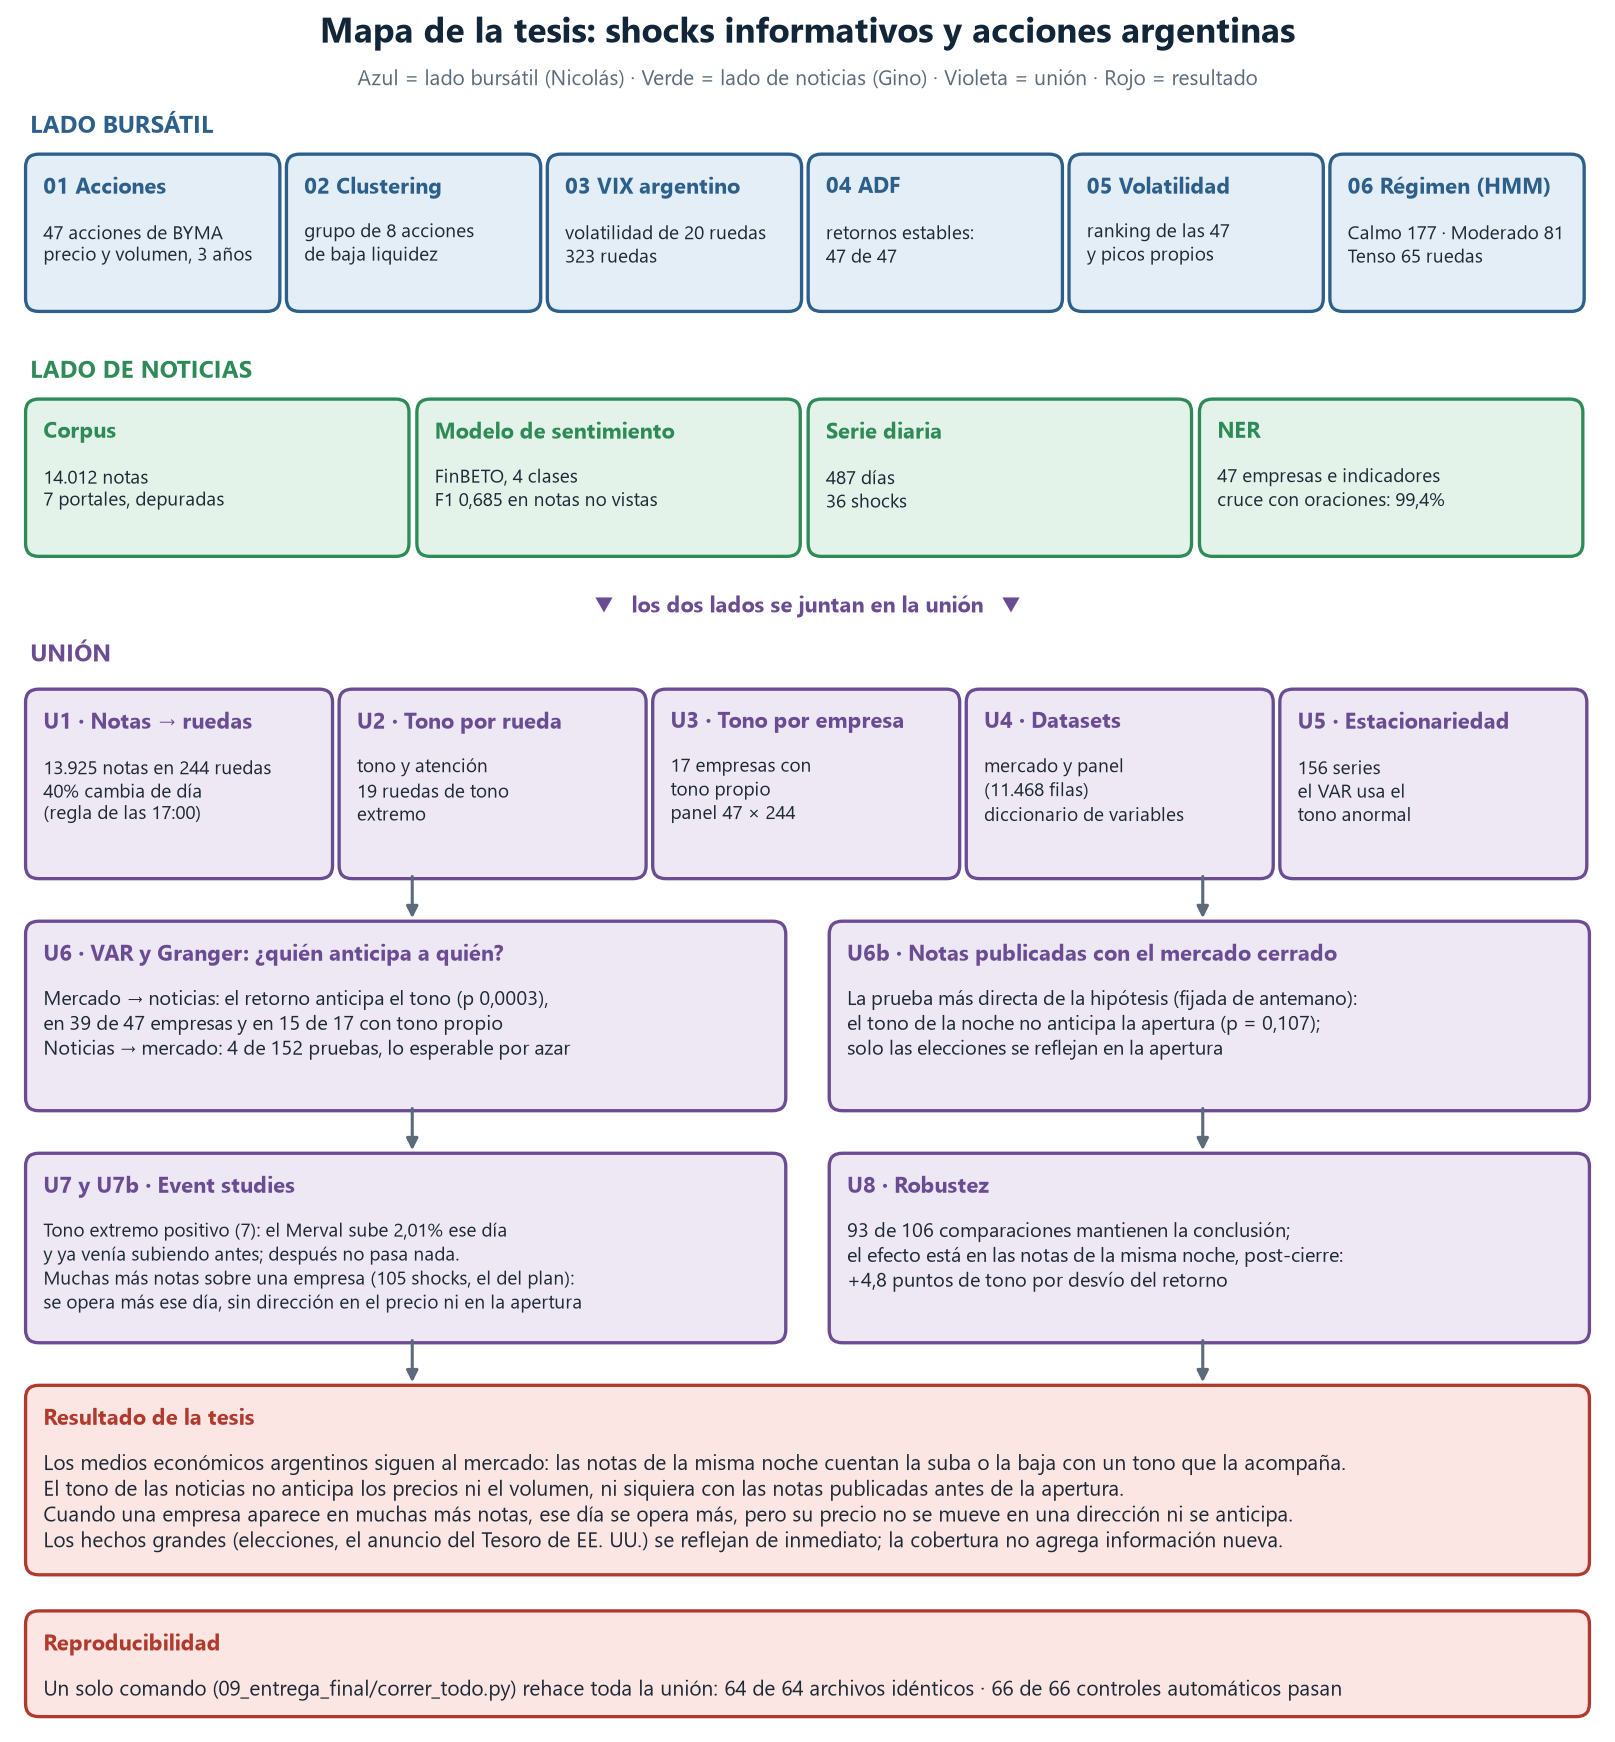
\includegraphics[width=0.6\linewidth]{mapa_tesis.png}
\caption{Mapa de la tesina: el lado bursátil (azul), el lado de noticias (verde), la unión
(violeta) y el resultado (rojo). Fuente: elaboración propia
(\carpeta{Unión/09_entrega_final/mapa_tesis.py}).}
\label{fig:mapa}
\end{figure}

% ---------------------------------------------------------------------
\section{Cuatro instrumentos y un experimento}

Los capítulos~\ref{cap:corpus} a~\ref{cap:hmm} presentan los cuatro instrumentos de medición que
hubo que construir: \textbf{el corpus de noticias} (capítulo~\ref{cap:corpus}); \textbf{FinBETO,
el termómetro emocional} de las noticias, con el reconocimiento de entidades que da el tono de
cada empresa (capítulo~\ref{cap:finbeto}); \textbf{el VIX argentino}, que mide la tensión del
mercado, junto con el panel de acciones (capítulo~\ref{cap:vix}); y \textbf{los regímenes de
mercado} estimados con un modelo oculto de Markov (capítulo~\ref{cap:hmm}). El
capítulo~\ref{cap:var} usa los cuatro en el experimento que contrasta la hipótesis: modelos VAR y
pruebas de causalidad de Granger en las dos direcciones. Que los instrumentos estén validados es
lo que permite leer con confianza el resultado: si el termómetro mide bien y aun así el tono no
anticipa al mercado, la ausencia de efecto es un hallazgo y no una falla de medición.

% =====================================================================
\chapter{Marco teórico}
\label{cap:marco}

Que «las noticias mueven la bolsa» mezcla dos ideas: que el precio cambia cuando llega
información nueva, y que los medios son el vehículo de esa información. Pero los medios también
informan sobre el propio mercado: una nota que cuenta que «el Merval subió 5\%» tiene tono
positivo, y su causa es el precio, no al revés. Este capítulo presenta los conceptos con los que
se analiza esa doble relación.

\textbf{Shock informativo y eficiencia.} Un \textit{shock informativo} es la llegada de
información que se aparta de lo esperado. La cantidad de noticias capta la \textit{atención}
\citep{da2011,fang2009}; el tono capta el \textit{contenido} \citep{tetlock2007,ardia2022}. La
hipótesis de mercados eficientes \citep{fama1970} sostiene que la información pública se
incorpora al precio tan rápido que no sirve para anticiparlo, y que el precio sigue un paseo
aleatorio. La evidencia para Argentina y la región es mixta \citep{zablotsky2002}.

\textbf{Sentimiento y tono de los medios.} El sentimiento del inversor es el optimismo o
pesimismo que no se explica por los fundamentos. Un tono muy pesimista anticipa bajas
transitorias \citep{tetlock2007}, sobre todo en las recesiones \citep{garcia2013}; pero el tono
también puede ser un \textit{reflejo} del mercado \citep{verma2026}. La tabla~\ref{tab:mecanismos}
resume cómo se reconoce cada dirección en los datos.

\begin{table}[H]
\centering\small
\begin{tabularx}{\linewidth}{@{}L{2.8cm}YY@{}}
\toprule
 & \textbf{Noticias \flecha{} mercado} & \textbf{Mercado \flecha{} noticias} \\
\midrule
Mecanismo & La nota trae información nueva o mueve el ánimo de los inversores & La nota cuenta lo que el mercado ya hizo \\
Qué se espera ver & El tono anticipa el retorno o el volumen de las ruedas siguientes & El retorno anticipa el tono de las notas siguientes \\
En un estudio de eventos & El retorno anormal aparece el día del evento o después & El retorno anormal aparece antes del evento \\
Con notas de la noche & El tono de la noche anticipa el salto de apertura & El tono de la noche refleja el cierre del día \\
\bottomrule
\end{tabularx}
\caption{Las dos direcciones de la relación entre noticias y mercado y cómo se reconoce cada
una en los datos. Fuente: elaboración propia.}
\label{tab:mecanismos}
\end{table}

\textbf{Volatilidad y regímenes.} La volatilidad se agrupa en períodos de calma y de estrés, lo
que para el S\&P~Merval está documentado con modelos GARCH \citep{segovia2022}; las caídas pesan
más que las subas \citep{otuki2008}. Una forma de describir esa alternancia es suponer que el
mercado pasa por unos pocos \textit{regímenes} y salta de uno a otro según una cadena de Markov
\citep{hamilton1989,rabiner1989}, un enfoque aplicado también en Latinoamérica
\citep{ataurima2016}. El régimen importa porque la relación entre noticias y precios podría
cambiar según el mercado esté calmo o tenso \citep{garcia2013}.

\textbf{Causalidad de Granger y VAR.} Con datos observacionales no se prueba una causa, pero sí
qué variable se mueve antes. $X$ \textit{causa en sentido de Granger} a $Y$ si el pasado de $X$
mejora la predicción de $Y$ más allá de su propio pasado \citep{granger1969}. La prueba se hace
dentro de un vector autorregresivo (VAR), que explica cada variable con los rezagos de todas y
trata las dos direcciones de forma simétrica \citep{sims1980,lutkepohl2005}.

\textbf{Estudios de eventos.} Miden qué hace el precio alrededor de un hecho puntual, comparado
con lo que habría sido normal \citep{mackinlay1997}: si la noticia mueve el mercado, el retorno
anormal aparece el día del evento o después; si lo refleja, aparece antes.

\textbf{Unidades de análisis.} Las 47 acciones del panel pertenecen a diez sectores: Consumo (9),
Financiero (8), Utilities (8), Materiales (6), Energía (4), Conglomerado, Industrial y Real Estate
(3 cada uno), Comunicaciones (2) y Tecnología (1). Para medir el tono propio de una empresa hace
falta que tenga noticias en buena parte de las ruedas; con un corte de 90 de las 244 ruedas
quedan 17: YPFD, BBAR, SUPV, EDN, GGAL, CEPU, TGSU2, IRSA, BMA, LOMA, PAMP, CRES, BYMA, TRAN,
METR, TXAR y ALUA (cualquier corte entre 75 y 94 da las mismas). Las noticias vienen de siete
portales nacionales, cada uno con su propio tono promedio (de +30,4 puntos en TN a 0,0 en Ámbito
Finanzas), lo que obliga a controlar la composición por portal.

% =====================================================================
\chapter{Primer instrumento: el corpus de noticias}
\chaptermark{El corpus de noticias}
\label{cap:corpus}

Para medir el tono de la prensa económica primero hay que tenerla. No existe un archivo
público y ordenado de las notas de economía de los portales argentinos, así que el corpus se
construyó con \textit{web scraping}: la extracción automática de información de páginas web.
Este capítulo describe cómo se recolectó, cómo se auditó y cómo se ordenó cada nota en el
tiempo del mercado.

% ---------------------------------------------------------------------
\section{Recolección}
\label{sec:recoleccion}

Para un corpus histórico de noticias hay dos caminos, y se usaron los dos según la
disponibilidad de cada portal:

\begin{itemize}
  \item \textbf{Internet Archive.} Su \textit{Wayback Machine} guarda capturas de millones de
        páginas, y su API CDX permite listar las capturas de un sitio en un rango de fechas.
        Así se puede reconstruir una ventana más larga que la que exponen los propios portales,
        a costa de depender de qué capturó un tercero \citep{garg2025wayback}. Se usó para
        Ámbito Financiero (Economía y Finanzas), Clarín (Economía), Infobae, La Nación y TN.
  \item \textbf{Mapas del sitio.} Los portales publican archivos \texttt{sitemap.xml} para los
        buscadores, que listan sus notas recientes. Se usaron para Clarín, El Economista e
        iProfesional. Clarín se cubrió con ambos métodos: la ventana más profunda por la
        Wayback Machine y las notas más recientes por el mapa del sitio.
\end{itemize}

Una vez obtenida la página, hay que separar el texto de la nota del «relleno» (menús,
publicidad, firmas) y extraer sus metadatos. Se usó una estrategia en capas: los datos
estructurados JSON-LD primero, después las metaetiquetas Open Graph, el título
\texttt{<h1>}, la librería \texttt{trafilatura} \citep{barbaresi2021} y, como último recurso,
reglas sobre el HTML con BeautifulSoup. Cada nota se guardó con su sitio, fecha y hora de
publicación, título, bajada, contenido y etiquetas. El acceso autenticado a la API de Internet
Archive usa credenciales guardadas en un archivo de configuración externo, fuera del código.

El corpus final tiene \textbf{14.012 artículos} de siete portales, recolectados en nueve
fuentes (tabla~\ref{tab:corpus}): unos 63 millones de caracteres, alrededor de 4.500 por
artículo. Aunque abarca de enero de 2025 a mayo de 2026, en la práctica empieza en mayo de
2025: 14.001 de las 14.012 notas son del 1 de mayo de 2025 en adelante, porque tanto la
retención de los mapas del sitio como las capturas de la Wayback Machine se concentran en los
meses más recientes.

\begin{table}[H]
\centering\small
\begin{tabular}{@{}llr@{}}
\toprule
\textbf{Portal} & \textbf{Método de recolección} & \textbf{Artículos} \\
\midrule
iProfesional & Mapa del sitio & 5.455 \\
Clarín & Mapa del sitio & 3.737 \\
Clarín — Economía & Wayback Machine & 294 \\
El Economista & Mapa del sitio & 2.695 \\
Ámbito Financiero — Economía & Wayback Machine & 498 \\
Ámbito Financiero — Finanzas & Wayback Machine & 240 \\
Infobae — Economía & Wayback Machine & 500 \\
La Nación — Economía & Wayback Machine & 491 \\
TN — Economía & Wayback Machine & 102 \\
\midrule
\textbf{Total} & & \textbf{14.012} \\
\bottomrule
\end{tabular}
\caption{Corpus de noticias por fuente, después de la depuración. Fuente: elaboración propia
(\carpeta{Lado Noticias/noticias}).}
\label{tab:corpus}
\end{table}

% ---------------------------------------------------------------------
\section{Auditoría y depuración}

Las herramientas de extracción de contenido fallan con frecuencia en el relleno y en los
metadatos \citep{foley2026wcxb}, por lo que un corpus web tiene que auditarse antes de usarse:
buscar plantillas, duplicados y contenido que no corresponde \citep{dodge2021c4}. Los
duplicados, además, distorsionan cualquier modelo que se entrene con ese texto
\citep{lee2021dedup}. La auditoría encontró cinco problemas, cada uno con su solución
(tabla~\ref{tab:depuracion}).

\begin{table}[H]
\centering\small
\begin{tabularx}{\linewidth}{@{}L{3.4cm}YY@{}}
\toprule
\textbf{Problema} & \textbf{Qué se encontró} & \textbf{Solución} \\
\midrule
Duplicados exactos & 205 notas de Clarín descargadas dos veces, por Wayback Machine y por el mapa del sitio & Una copia por URL (la del sitio); los recolectores verifican la URL contra todo el corpus \\
Publicación cruzada & 208 grupos de título repetido; 175 se descartaron por estar a más de 48 horas (columnas recurrentes) & Los 33 grupos restantes (68 notas) se verificaron con Qwen3: 14 republicaciones reales \\
Metadatos faltantes & Sin autor ni palabras clave en iProfesional y sin fecha en 194 notas de El Economista, por un error de parseo del JSON-LD & Parseo tolerante; 192 notas reales se volvieron a descargar y recuperaron su fecha \\
Contenido que no es noticia & 2 páginas índice, 9 páginas de suscripción y 6 notas fuera de la ventana (fechadas por su última modificación) & Se eliminaron; los recolectores filtran por fecha de publicación efectiva \\
Plantillas & 65 grupos (479 notas) con el mismo comienzo; cuatro plantillas de El Economista concentran 325 notas con sentimiento constante & Se eliminaron 419 notas (2,9\%): el corpus pasó de 14.431 a 14.012 \\
\bottomrule
\end{tabularx}
\caption{Problemas del corpus y cómo se resolvieron. Fuente: elaboración propia a partir de
la auditoría del lado de noticias (\carpeta{Lado Noticias/noticias}).}
\label{tab:depuracion}
\end{table}

Las plantillas merecen un comentario, porque muestran por qué la auditoría es parte del
instrumento y no un trámite. Notas como el reporte diario «Dólar hoy» tienen fecha y
cotizaciones propias, pero el modelo de sentimiento les asignaba siempre el mismo valor, con
desvío cero entre decenas de notas: el valor dependía de la parte fija del texto y no de la
información del día. Replicado durante meses, ese valor sesgaba el promedio diario. En los
grupos de menos de 11 notas se conservó la más antigua (83 eliminadas); en los de 11 o más,
cuyo cuerpo es relleno, se eliminaron todas (336). Una sola nota de 2014 mal fechada, además,
estiraba la serie diaria a 4.186 días; tras la depuración la serie abarca 487 días. La
verificación de duplicados semánticos se hizo con el modelo de lenguaje abierto Qwen3, servido
localmente con Ollama.

% ---------------------------------------------------------------------
\section{Cada nota a su rueda}
\label{sec:alineacion}

Las noticias se publican a cualquier hora, pero el precio se forma solo en las ruedas, de lunes
a viernes de 11:00 a 17:00. Para medir si una nota mueve el precio hay que compararla con el
primer precio que pudo verse afectado por ella: una nota del martes a las 20:00 sale con el
mercado cerrado, y la primera vez que alguien puede operar con esa información es el miércoles.
Se aplicó la siguiente regla:

\begin{itemize}
  \item Todas las horas se pasaron a hora argentina: Clarín, Infobae y La Nación informan la
        hora en UTC, y 95 notas nocturnas cambian de fecha con la conversión.
  \item Una nota publicada antes de las 17:00 de un día con rueda cuenta para esa rueda.
  \item Una nota publicada a las 17:00 o después cuenta para la rueda siguiente.
  \item Una nota publicada en un día sin rueda (fin de semana o feriado) cuenta para la
        primera rueda posterior.
\end{itemize}

Dentro de la ventana común con el mercado (05/05/2025 al 30/04/2026, 244 ruedas) quedaron
13.925 notas (tabla~\ref{tab:alineacion}); las 10 de enero a marzo de 2025 y las 77 del cierre
del 30/04/2026 en adelante quedan afuera. Las 244 ruedas reciben noticias: mínimo 12, mediana 55
y máximo 145. Los lunes reciben el fin de semana: mediana de 85 notas, contra 50 el resto de los
días (figura~\ref{fig:u1}).

\begin{table}[H]
\centering\small
\begin{tabular}{@{}lrr@{}}
\toprule
\textbf{Dónde quedó cada nota} & \textbf{Notas} & \textbf{\%} \\
\midrule
En su mismo día (antes de las 17:00 de un día con rueda) & 8.332 & 59,8 \\
En la rueda siguiente, por salir después del cierre & 3.451 & 24,8 \\
En la rueda siguiente, por salir en un día sin rueda & 2.142 & 15,4 \\
\midrule
Total dentro de la ventana & 13.925 & 100,0 \\
\bottomrule
\end{tabular}
\caption{Asignación de las notas a las ruedas con la regla de las 17:00. Fuente: elaboración
propia (\carpeta{Unión/01_alineacion_noticias_ruedas}).}
\label{tab:alineacion}
\end{table}

\begin{figure}[H]
\centering
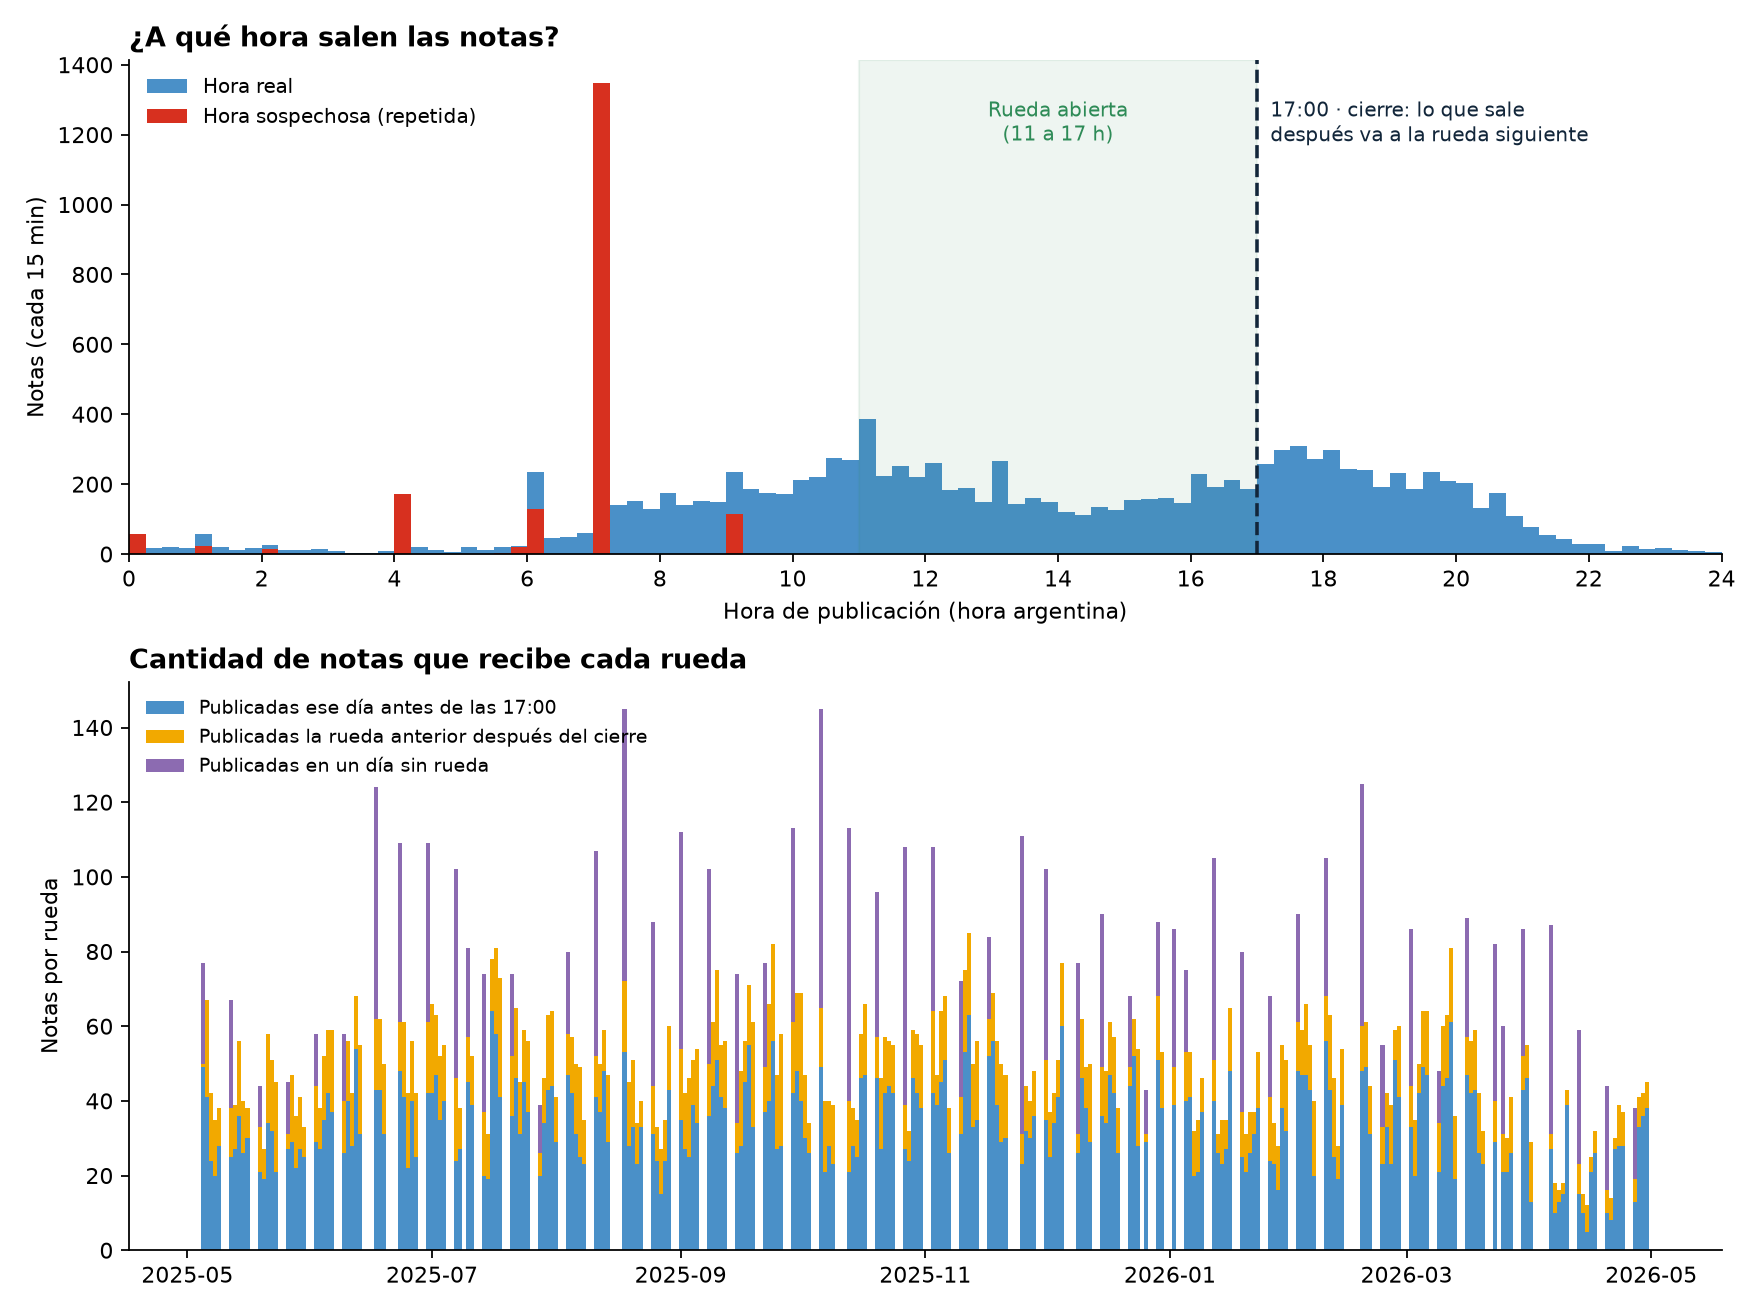
\includegraphics[width=0.76\linewidth]{u1_alineacion_reducida.png}
\caption{Arriba: hora de publicación de las notas, con la rueda sombreada y el cierre de las
17:00; en rojo, horas repetidas que no pueden ser reales. Abajo: notas que recibe cada rueda,
según de dónde vienen. Fuente: elaboración propia (\carpeta{Unión/01_alineacion_noticias_ruedas}).}
\label{fig:u1}
\end{figure}

\textbf{Horas sospechosas.} El 13,4\% de las notas (1.881) tiene una hora que se repite
demasiado dentro de su portal —más del 3\% de sus notas a un mismo minuto—, como las 07:00 de
Clarín o las 00:00 de Ámbito. No es la hora real sino una hora por defecto del sitio. Esas
notas se marcaron y los resultados se repitieron sin ellas (sección~\ref{sec:var-robustez}). La
alineación pasó 10 controles automáticos: por ejemplo, ninguna nota va a una rueda anterior a su
publicación, y ninguna publicada tras el cierre queda en la rueda del mismo día.

\textbf{Límites del instrumento.} La cobertura depende de qué capturó la Wayback Machine y de
la retención de los mapas del sitio; abril de 2026 tiene un hueco de recolección en
iProfesional, el portal más grande, y se marcó para analizarlo aparte. Las notas pertenecen a
sus medios y se usaron únicamente con fines académicos: el análisis trabaja con medidas
agregadas (tono, cantidad, menciones) y no reproduce las notas.

% =====================================================================
\chapter{Segundo instrumento: FinBETO, el termómetro emocional}
\chaptermark{FinBETO, el termómetro emocional}
\label{cap:finbeto}

El corpus dice qué se publicó; falta saber con qué tono. Para eso se construyó FinBETO, un
modelo de lenguaje que lee cada oración de una nota y la clasifica como positiva, negativa,
neutra o mixta. Agregadas por rueda, esas clasificaciones dan una medida de la temperatura
emocional de la prensa económica: cuán optimistas o pesimistas fueron las noticias de cada día.

% ---------------------------------------------------------------------
\section{De BERT a FinBETO}

BERT \citep{devlin2019bert} es un modelo de lenguaje preentrenado con la tarea de adivinar
palabras ocultas en un texto (\textit{masked language modeling}, MLM). BETO es su versión
entrenada en español \citep{canete2020beto}. Para clasificar sentimiento se le agrega una capa
de salida y se lo ajusta con oraciones etiquetadas (\textit{fine-tuning}), como hizo FinBERT en
inglés \citep{araci2019finbert}. Antes del ajuste conviene seguir el preentrenamiento con texto
del propio dominio, porque mejora el desempeño en la tarea final \citep{gururangan2020dapt}.
FinBETO es el resultado de los dos pasos sobre la prensa económica argentina.

\textbf{Clases.} Se trabajó con cuatro: positiva (POS), negativa (NEG), neutra (NEU) y mixta
(MIXTO). Una parte de las oraciones de la prensa económica combina señales de ambos signos —por
ejemplo, un dato de actividad que mejora mientras la inflación se acelera— y forzarlas a una
sola clase habría sido arbitrario.

% ---------------------------------------------------------------------
\section{Etiquetado y entrenamiento}

\textbf{Etiquetado con Gemma.} Para el ajuste fino hacen falta oraciones etiquetadas, y no
existía un conjunto público de prensa económica argentina. Se usó un modelo de lenguaje como
etiquetador, una práctica que puede igualar o superar a anotadores contratados
\citep{gilardi2023chatgpt} y que también se evaluó en textos financieros
\citep{aguda2024llmannot}. El etiquetador fue Gemma \citep{gemma2026gemma4}
(\texttt{gemma4:26b}, temperatura 0,1), ejecutado localmente con Ollama, en dos pasos por
noticia. Primero leyó el título, la bajada y los primeros 3.000 caracteres, y produjo un
análisis de contexto (tema central, encuadre, actores y tono general). Después etiquetó cada
oración de al menos 30 caracteres, con ese contexto como referencia y la instrucción de que el
sentimiento surgiera de lo que la oración expresa por sí misma. Se tomó un artículo de cada una
de las nueve fuentes por lote, hasta 408 noticias (45 o 46 por fuente) y 11.605 oraciones
etiquetadas: 46,4\% NEU, 23,8\% POS, 20,8\% NEG y 8,9\% MIXTO.

\textbf{Preentrenamiento continuado.} Se hizo con la tarea MLM (15\% de los tokens
enmascarados) sobre el texto de los 14.667 artículos del corpus antes de su depuración final:
3 épocas, segmentos de 128 tokens y tasa de aprendizaje $2\cdot10^{-5}$. La pérdida de
evaluación bajó de 1,233 a 1,121, y ante la frase «La [MASK] llegó al 3\% mensual según el
INDEC» el modelo propuso «inflación» con probabilidad 0,81: ya hablaba el idioma de la prensa
económica argentina.

\textbf{Ajuste fino.} Para que la clase neutra no dominara, se tomó una muestra balanceada de
hasta 2.400 oraciones por clase (todas las de MIXTO), dividida en 80\% para entrenamiento,
10\% para validación y 10\% para prueba (6.588, 824 y 824 oraciones). Como aun así la clase
MIXTO tiene menos ejemplos que las demás, durante el entrenamiento un error en una clase escasa
se penalizó algo más que un error en una clase abundante: cuanto más rara es la clase, más pesa
cada uno de sus errores, aunque de forma moderada, para que el modelo no la ignore sin
exagerar su importancia\footnote{Técnicamente, la pérdida se ponderó por la raíz cuadrada de la
frecuencia inversa de cada clase.}. Se usaron 5 épocas, lotes de 32, tasa de aprendizaje
$2\cdot10^{-5}$ con 10\% de calentamiento, decaimiento de pesos 0,01 y selección de la mejor
época por F1 macro en validación. El F1 macro —el promedio simple del F1 de cada clase— es la
métrica principal, porque no premia acertar solo la clase más frecuente.

% ---------------------------------------------------------------------
\section{Evaluación: cuánto mide bien el termómetro}

La primera evaluación informó un F1 macro de 0,7296 en cuatro clases. Al revisarla se
encontraron tres problemas: la división de los datos se había hecho por oración y no por
noticia, de modo que las oraciones de prueba venían de noticias que también aportaban
oraciones al entrenamiento; había textos repetidos (41 oraciones de prueba, el 5\%, estaban
también en entrenamiento); y había restos del \textit{scraping} etiquetados como neutros
(«PUBLICIDAD PUBLICIDAD PUBLICIDAD», «Sobre la firma Newsletter Clarín»). Es el problema de
fuga de información descrito por \citet{kapoor2023leakage}: con noticias, la forma de dividir
los datos cambia mucho el resultado \citep{xue2026temporal}.

Para medir bien, sin modificar el modelo en uso, se limpió el conjunto etiquetado (se
descartaron 750 filas de relleno o repetidas y quedaron 10.855 oraciones), se lo dividió
\textit{por noticia} (330 noticias para entrenamiento, 39 para validación y 39 para prueba,
sin textos compartidos) y se reentrenó solo para medir, con tres semillas por división. El
código reproduce el resultado original (0,732 con la división por oración); con la división
por noticia, el F1 macro es de \textbf{0,685} (tabla~\ref{tab:finbeto}). Esa es la estimación
honesta, porque el 97\% de las noticias del corpus nunca se vio al entrenar.

Para comparar en igualdad de condiciones con el modelo de referencia,
\carpeta{finiteautomata/beto-sentiment-analysis} \citep{perez2021pysentimiento}, un BETO
ajustado con tuits en tres clases, se usaron solo las oraciones POS, NEG y NEU, contando como
error cada predicción MIXTO de FinBETO. Sobre noticias no vistas, FinBETO obtiene
\textbf{0,724} y el de referencia \textbf{0,546}: 17,7 puntos de ventaja. El de referencia
clasifica como neutras 411 de las 662 oraciones; el ajuste al dominio es lo que le permite a
FinBETO leer el tono de la prensa económica.

\begin{table}[H]
\centering\footnotesize
\begin{tabular}{@{}lcc@{}}
\toprule
\textbf{Medida (prueba, media de 3 semillas)} & \textbf{División por oración} & \textbf{División por noticia} \\
\midrule
F1 macro, 4 clases & 0,732 $\pm$ 0,012 & \textbf{0,685 $\pm$ 0,009} \\
Exactitud & 0,743 & 0,691 \\
F1 POS / NEG / NEU / MIXTO & 0,752 / 0,760 / 0,754 / 0,663 & 0,694 / 0,677 / 0,725 / 0,645 \\
\midrule
F1 macro, 3 clases: FinBETO & 0,773 & \textbf{0,724} \\
F1 macro, 3 clases: modelo de referencia & 0,620 & 0,546 \\
\bottomrule
\end{tabular}
\caption{Calidad de FinBETO según cómo se dividen los datos. La estimación que corresponde
informar es la de la división por noticia. Fuente: elaboración propia a partir de
\carpeta{Lado Noticias/sentimiento_finbert}.}
\label{tab:finbeto}
\end{table}

% ---------------------------------------------------------------------

\section{Del modelo a la temperatura de cada rueda}
\label{sec:tono-rueda}

El modelo se aplicó a todas las oraciones del corpus de entre 30 y 600 caracteres, incluido el
título. Se excluyeron 2.438 oraciones de relleno (firmas de Clarín, marcas de publicidad de
Infobae) y quedaron 399.803: 36,7\% neutras, 27,1\% positivas, 24,1\% negativas y 12,1\%
mixtas. Para cada nota se calculó el \textit{sentimiento neto}: el porcentaje de oraciones
positivas menos el de negativas; las mixtas y las neutras no suman ni restan. Con cada nota ya
asignada a su rueda (sección~\ref{sec:alineacion}) se armaron cuatro medidas:

\begin{itemize}
  \item \textbf{Tono:} el promedio del sentimiento neto de las notas de la rueda, también en una
        versión \textit{ajustada por portal} (correlación 0,995 con la original).
  \item \textbf{Tono anormal:} el tono de la rueda menos el promedio de las 20 ruedas previas.
        Mide la sorpresa en lugar del clima de fondo, y es la variable de tono de los modelos.
  \item \textbf{Atención:} la cantidad de notas de la rueda comparada con lo habitual, primero
        con las ruedas que cubren los mismos días (un lunes junta el fin de semana) y después
        con las 20 previas. En la \textit{atención anormal}, 0 es lo habitual, $+0{,}69$ el doble
        de notas y $-0{,}69$ la mitad.
  \item \textbf{Ruedas de tono extremo:} se compararon dos familias de reglas contra el azar,
        mezclando las notas entre las ruedas. La regla por desvío de los días previos marca casi
        lo mismo que el azar (15 shocks contra 16,1 con umbral 2). La regla \textit{por
        muestreo}, que tiene en cuenta cuántas notas tiene cada rueda, marca con umbral 2,5
        \textbf{19 ruedas} (10 positivas y 9 negativas) contra 3,5 del azar, y fue la elegida.
        La regla de la serie diaria original incluía al propio día en su ventana, lo que acota
        el desvío máximo a 2,27 \citep{shiffler1988}; por eso la unión la redefinió.
\end{itemize}

El termómetro tiene una lectura clara (figura~\ref{fig:u2}). El tono medio de las 244 ruedas
fue de 3,9 puntos, con un desvío de 7,0: las noticias económicas son, en promedio, levemente
positivas. La rueda más negativa fue la del 15/04/2026 ($-13{,}5$) y la más positiva, la del
14/11/2025 ($+22{,}1$). El tono de una rueda se parece al de la anterior: la correlación entre el
tono de cada rueda y el de la rueda previa es de 0,47. Si un día las noticias son más positivas
que lo habitual, al día siguiente tienden a seguir siéndolo, aunque en menor medida: el clima de
las noticias cambia de a poco, porque los temas se sostienen varios días en los medios.

\begin{figure}[H]
\centering
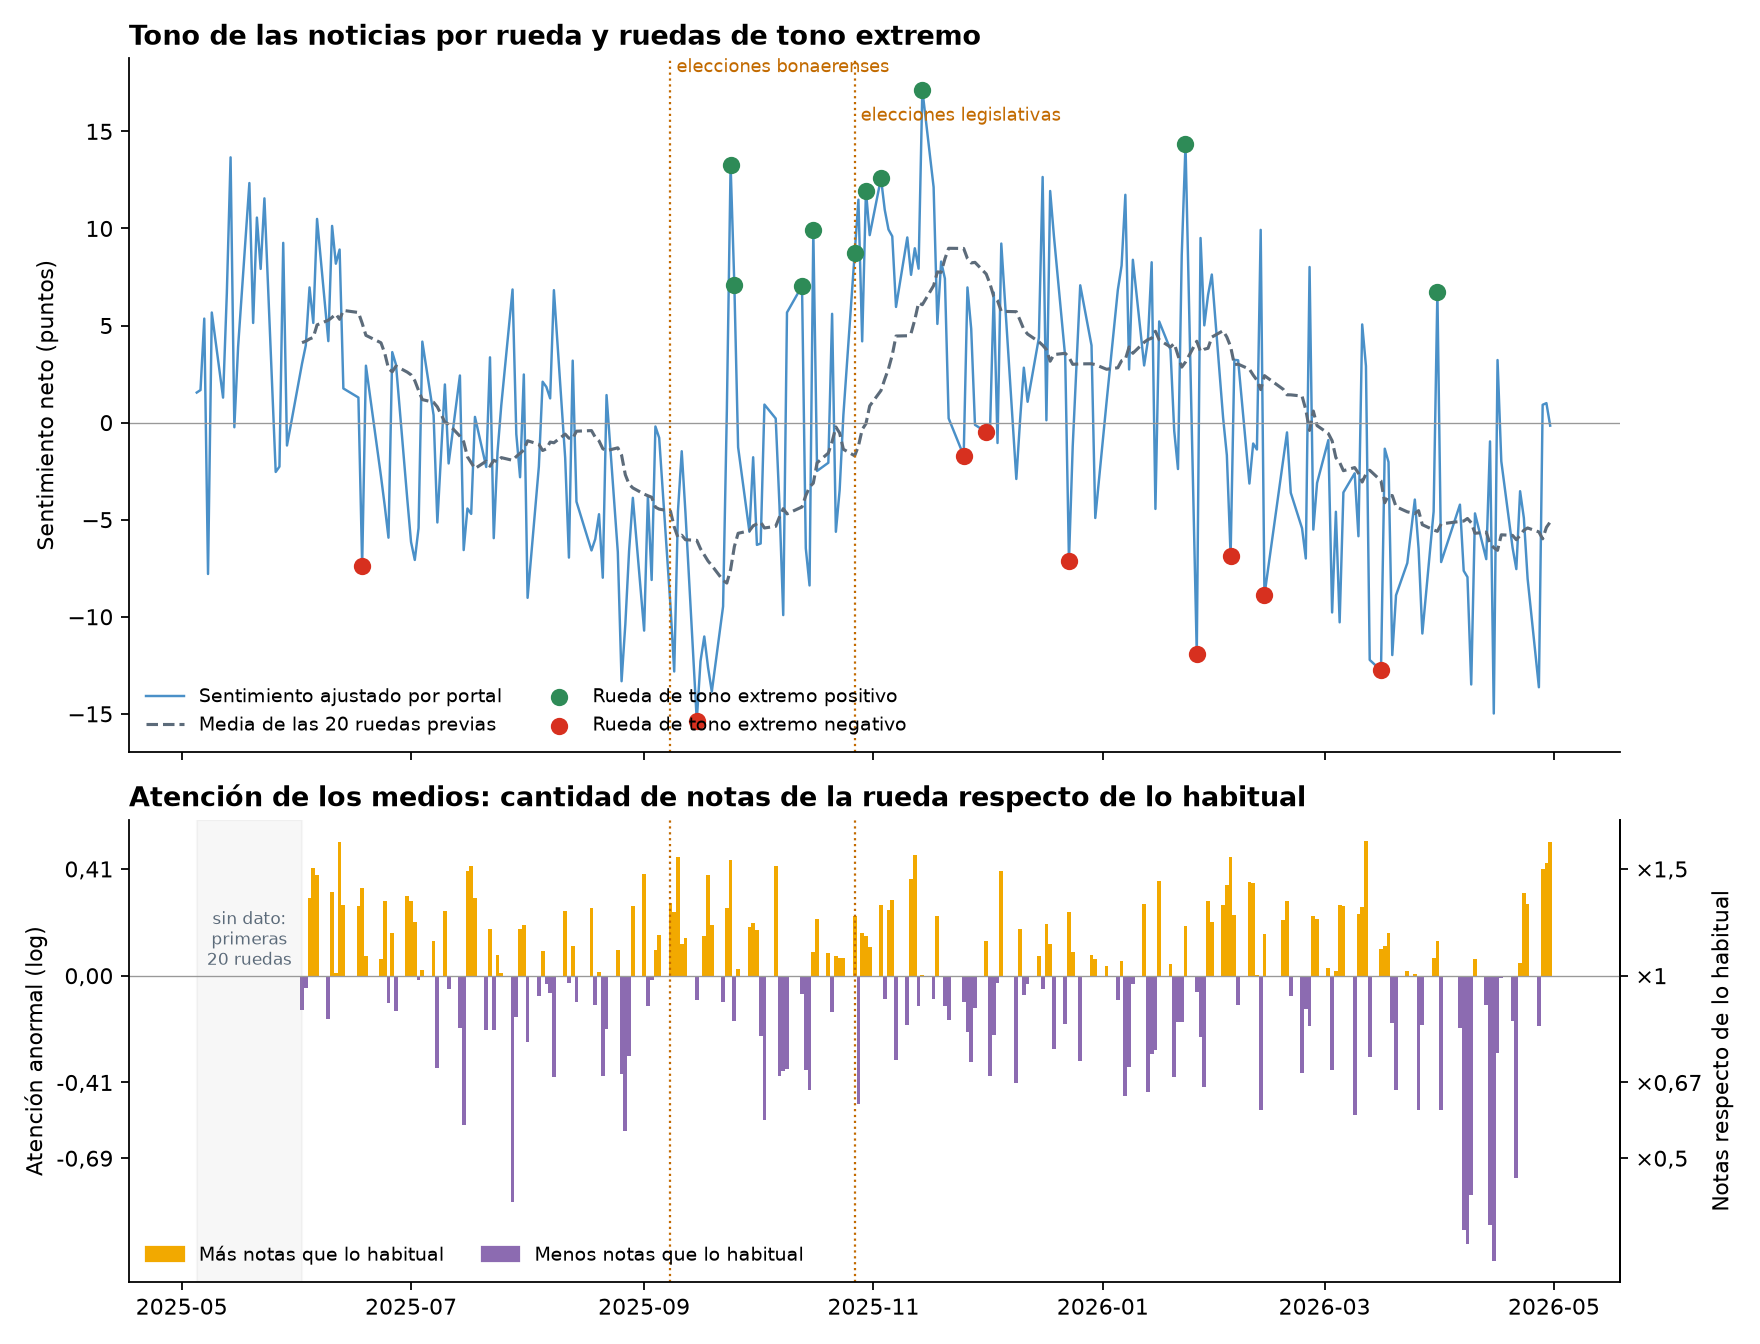
\includegraphics[width=0.74\linewidth]{u2_serie_reducida.png}
\caption{Arriba: tono de cada rueda (ajustado por portal), su media de las 20 ruedas previas y
las ruedas de tono extremo (verde, positivas; rojo, negativas); las líneas punteadas son los
días electorales. Abajo: atención de los medios, es decir, cuántas notas recibió cada rueda
respecto de lo habitual. Las barras naranjas son ruedas con más notas que lo habitual y las
violetas, con menos; el eje derecho traduce la escala a veces lo habitual ($\times 1{,}5$ es un
50\% más de notas, $\times 0{,}5$ la mitad). Las primeras 20 ruedas no tienen referencia previa.
Fuente: elaboración propia (\carpeta{Unión/02_sentimiento_por_rueda}).}
\label{fig:u2}
\end{figure}

% ---------------------------------------------------------------------
\section{Reconocimiento de entidades: el tono de cada empresa}
\label{sec:ner-modelo}

El termómetro mide el tono de las noticias en general. Para saber de qué empresa habla cada
oración se usó el reconocimiento de entidades nombradas (NER), que identifica nombres de
personas, organizaciones y lugares en un texto \citep{tjongkimsang2002conll}.

\textbf{Un NER híbrido.} Se combinó el modelo \texttt{es\_core\_news\_lg} de spaCy
\citep{honnibal2020spacy} con dos \textit{gazetteers} (diccionarios curados): 160 indicadores
económicos en seis categorías y las 47 empresas del panel, \textit{canonicalizadas}: cada alias
se resuelve al ticker, para que «Banco Galicia», «Grupo Financiero Galicia» y «GGAL» cuenten como
una sola entidad. Los alias en mayúsculas se buscan respetando mayúsculas (sin esa regla, AGRO
coincidía con «agro» en 920 artículos) y se excluyeron los que son palabras comunes
(«Hipotecario», «Molinos»). La limpieza quitó el relleno del \textit{scraping}, las
autorreferencias de cada medio y los fragmentos sin valor que detecta el modelo
(tabla~\ref{tab:ner}).

\begin{table}[H]
\centering\footnotesize
\begin{tabular}{@{}lll@{}}
\toprule
 & \textbf{Antes del filtrado} & \textbf{Después} \\
\midrule
Entidades únicas & 65.352 & 17.894 \\
«PUBLICIDAD» como entidad & 2.258 menciones (primera del ranking) & 0 \\
Empresas del panel & 20, fragmentadas en variantes & 47, canonicalizadas por ticker \\
Falsos positivos del alias AGRO & 920 artículos & 0 \\
\bottomrule
\end{tabular}
\caption{Efecto de la limpieza del reconocimiento de entidades. Fuente: elaboración propia a
partir de \carpeta{Lado Noticias/ner_entidades}.}
\label{tab:ner}
\end{table}

\textbf{Cruce con el sentimiento.} Cada mención se unió con el sentimiento FinBETO de su oración,
exigiendo que el texto coincida: se cruzaron el 99,37\% de las oraciones con entidades del corpus
(243.265 de 244.809). Antes de agregar, 24 variantes de indicadores se unificaron («PIB» y
«producto bruto interno» en «PBI»). YPF es la empresa más mencionada (237 de las 244 ruedas),
seguida por BBVA, Supervielle, Edenor y Galicia; tres empresas del panel no tienen ninguna
mención (CAPX, FIPL y LONG). El sentimiento de las oraciones que nombran a una empresa es el tono
del contexto en que aparece, no una opinión sobre ella.

\textbf{El tono propio.} El tono de una empresa en una rueda es (oraciones positivas $-$
negativas) / oraciones que la mencionan $\times$ 100. Como la mediana es de dos oraciones por
rueda, y en el 37\% de las ruedas hay una sola, ese valor sale muchas veces todo o nada. Por eso
se lo \textit{encoge} hacia el tono del mercado según la cantidad de oraciones $n$
\citep{efron1975}:
\begin{equation}
\text{tono propio}_{i,t} = \frac{n_{i,t}}{n_{i,t} + 10{,}9}\,\bigl(\text{tono}_{i,t} - \text{tono}_{M,t}\bigr),
\end{equation}
de modo que con una oración pesa un 8\%, con diez un 48\% y con treinta un 73\%. El tono propio
mide cuánto mejor o peor se habla de la empresa que del mercado, vale 0 si no hay noticias de
ella y se calcula para las 17 empresas con noticias frecuentes (figura~\ref{fig:u3}).

\begin{figure}[H]
\centering
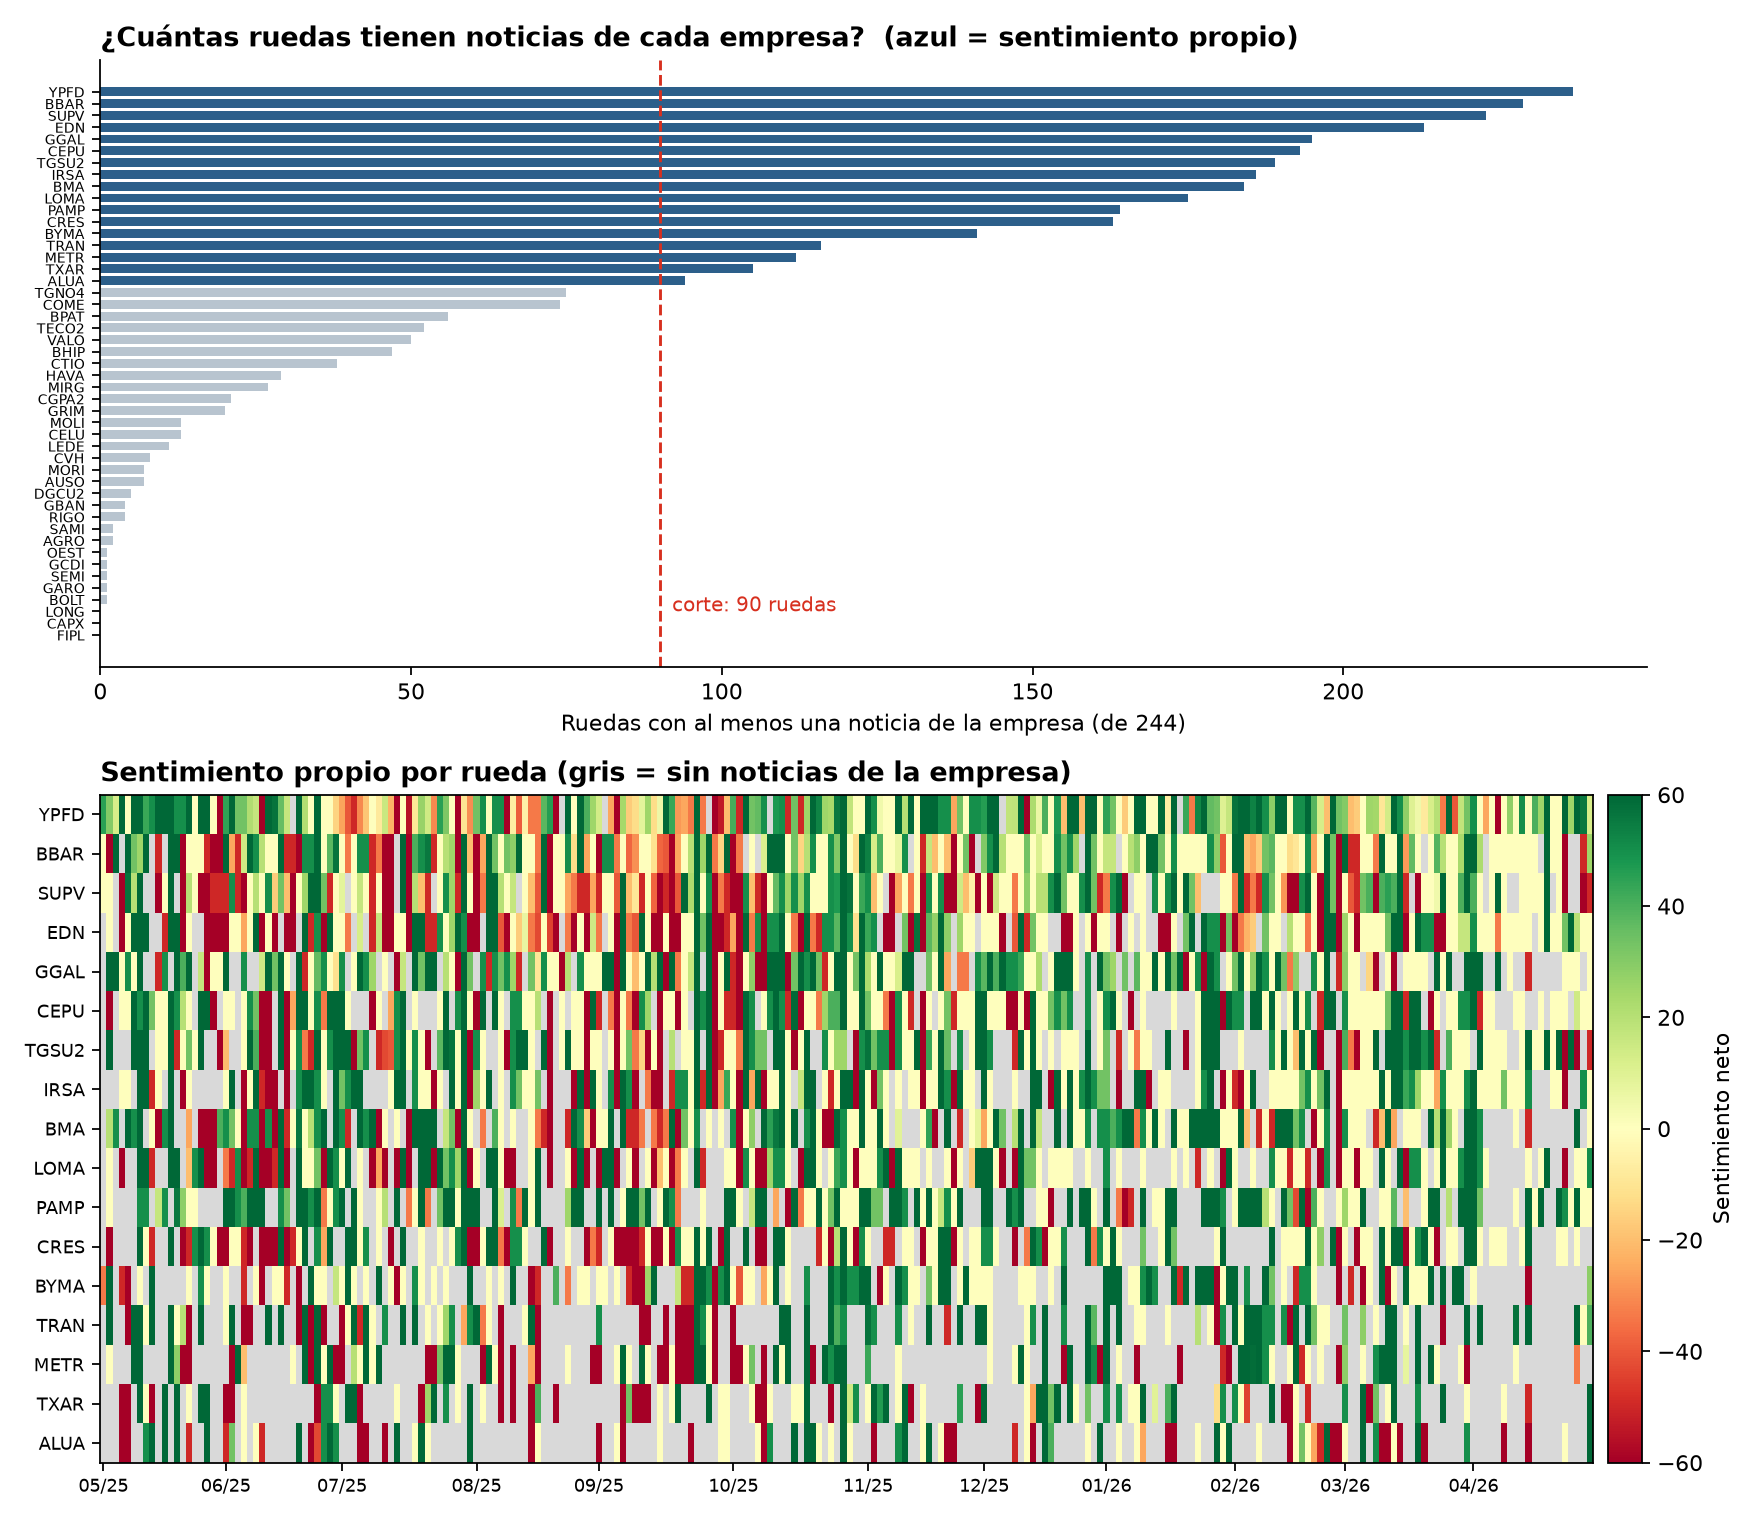
\includegraphics[width=0.55\linewidth]{u3_cobertura.png}
\caption{Arriba: ruedas con al menos una noticia de cada empresa (en azul, las 17 con tono
propio). Abajo: tono propio de esas 17 empresas en cada rueda. Fuente: elaboración propia
(\carpeta{Unión/03_sentimiento_por_empresa}).}
\label{fig:u3}
\end{figure}

% =====================================================================
\chapter{Tercer instrumento: el VIX argentino y el panel de acciones}
\chaptermark{El VIX argentino y el panel de acciones}
\label{cap:vix}

El VIX de Chicago es el termómetro más conocido del miedo en los mercados: sube cuando los
inversores esperan movimientos bruscos. Se calcula con precios de opciones, y en Argentina no
existe un mercado de opciones con la liquidez necesaria para construir algo así. Por eso se
construyó un \textit{VIX argentino} a partir de lo que sí está disponible todos los días: los
retornos del S\&P~Merval. Es el instrumento que mide cuánta tensión hay en el mercado, y la
base sobre la que se estiman los regímenes del capítulo~\ref{cap:hmm}. Este capítulo presenta
también el panel de acciones del lado bursátil: cómo se eligió, cómo se depuraron sus precios,
cuán volátil es cada acción y si las acciones forman familias de comportamiento.

% ---------------------------------------------------------------------
\section{El panel de acciones}
\label{sec:panel}

Los precios diarios (apertura, máximo, mínimo, cierre y volumen) se descargaron de Yahoo Finance
con \texttt{yfinance}. Se partió de 53 candidatas del Panel General y del Panel Líderes de BYMA
(las 20 del S\&P~Merval más 33 de sectores similares) y se exigieron dos condiciones en los tres
años de datos (731 ruedas): cobertura completa del calendario y al menos 90\% de días con volumen
real, porque un día sin operaciones no es un faltante sino una fila con el precio pegado. Pasaron
47, incluidas las 20 del índice; quedaron afuera Carboclor, Holcim, Polledo, Instituto Rosenbusch
y dos tickers sin datos (NII Holdings y TGLT, que hoy cotiza como GCDI). En la depuración se
quitaron las filas que Yahoo agrega en los feriados (se usó como calendario de BYMA la lista de
fechas del índice), se reintentaron los tickers con fallas intermitentes y se corrigieron dos
eventos corporativos mal ajustados: el \textit{split} de SEMI del 16/12/2024 y el dividendo en
acciones de AGRO de noviembre de 2023, que mostraba una caída falsa de 88\%.

% ---------------------------------------------------------------------
\section{Construcción del VIX argentino}

El VIX argentino es la \textit{volatilidad realizada} del índice: el desvío estándar de sus
retornos diarios en las últimas 20 ruedas, anualizado \citep{sakowski2023}:
\begin{equation}
\sigma_t = \sqrt{252}\cdot \operatorname{desv}\left(r_{t-19},\dots,r_t\right)\cdot 100,
\qquad r_t = \frac{P_t - P_{t-1}}{P_{t-1}},
\end{equation}
donde $P_t$ es el cierre del S\&P~Merval (\texttt{\^{}MERV} en Yahoo Finance) en la rueda $t$.
Veinte ruedas equivalen a un mes de operaciones, y el factor $\sqrt{252}$ es la convención
internacional de ruedas por año, que lleva el desvío diario a una escala anual comparable con
la de cualquier otro índice (BYMA tiene unas 244 ruedas por año por sus feriados; usar ese
número bajaría todos los valores un 1,5\%, sin cambiar ninguna comparación). Se calculó para la ventana del corpus de noticias: del 2 de enero
de 2025 al 30 de abril de 2026, 323 ruedas. El mismo cálculo, aplicado a cada acción, da su
volatilidad propia. La lista de fechas del índice se usó, además, como calendario de ruedas de
BYMA para todo el trabajo.

% ---------------------------------------------------------------------
\section{Cómo leer el gráfico}

La figura~\ref{fig:vix} tiene dos paneles que se leen juntos, y las líneas punteadas marcan los
tres hechos que dispararon la volatilidad del período: la salida del cepo y las dos elecciones. Arriba está el S\&P~Merval en
pesos: como los precios son nominales, su tendencia de fondo incluye la inflación y el tipo de
cambio, y lo que interesa son los saltos, no la pendiente. Abajo está el VIX argentino, con su
promedio del período (44,0\%) como referencia; el sombreado marca los días en que estuvo por
encima de ese promedio (136 de las 323 ruedas). Un VIX de 44\% quiere decir que, al ritmo del
último mes, el índice se movería en un año alrededor de un 44\% hacia arriba o hacia abajo. El
mínimo fue de 15,4\% el 30/04/2026 y el máximo, de 91,0\% el 21/11/2025.

\begin{figure}[H]
\centering
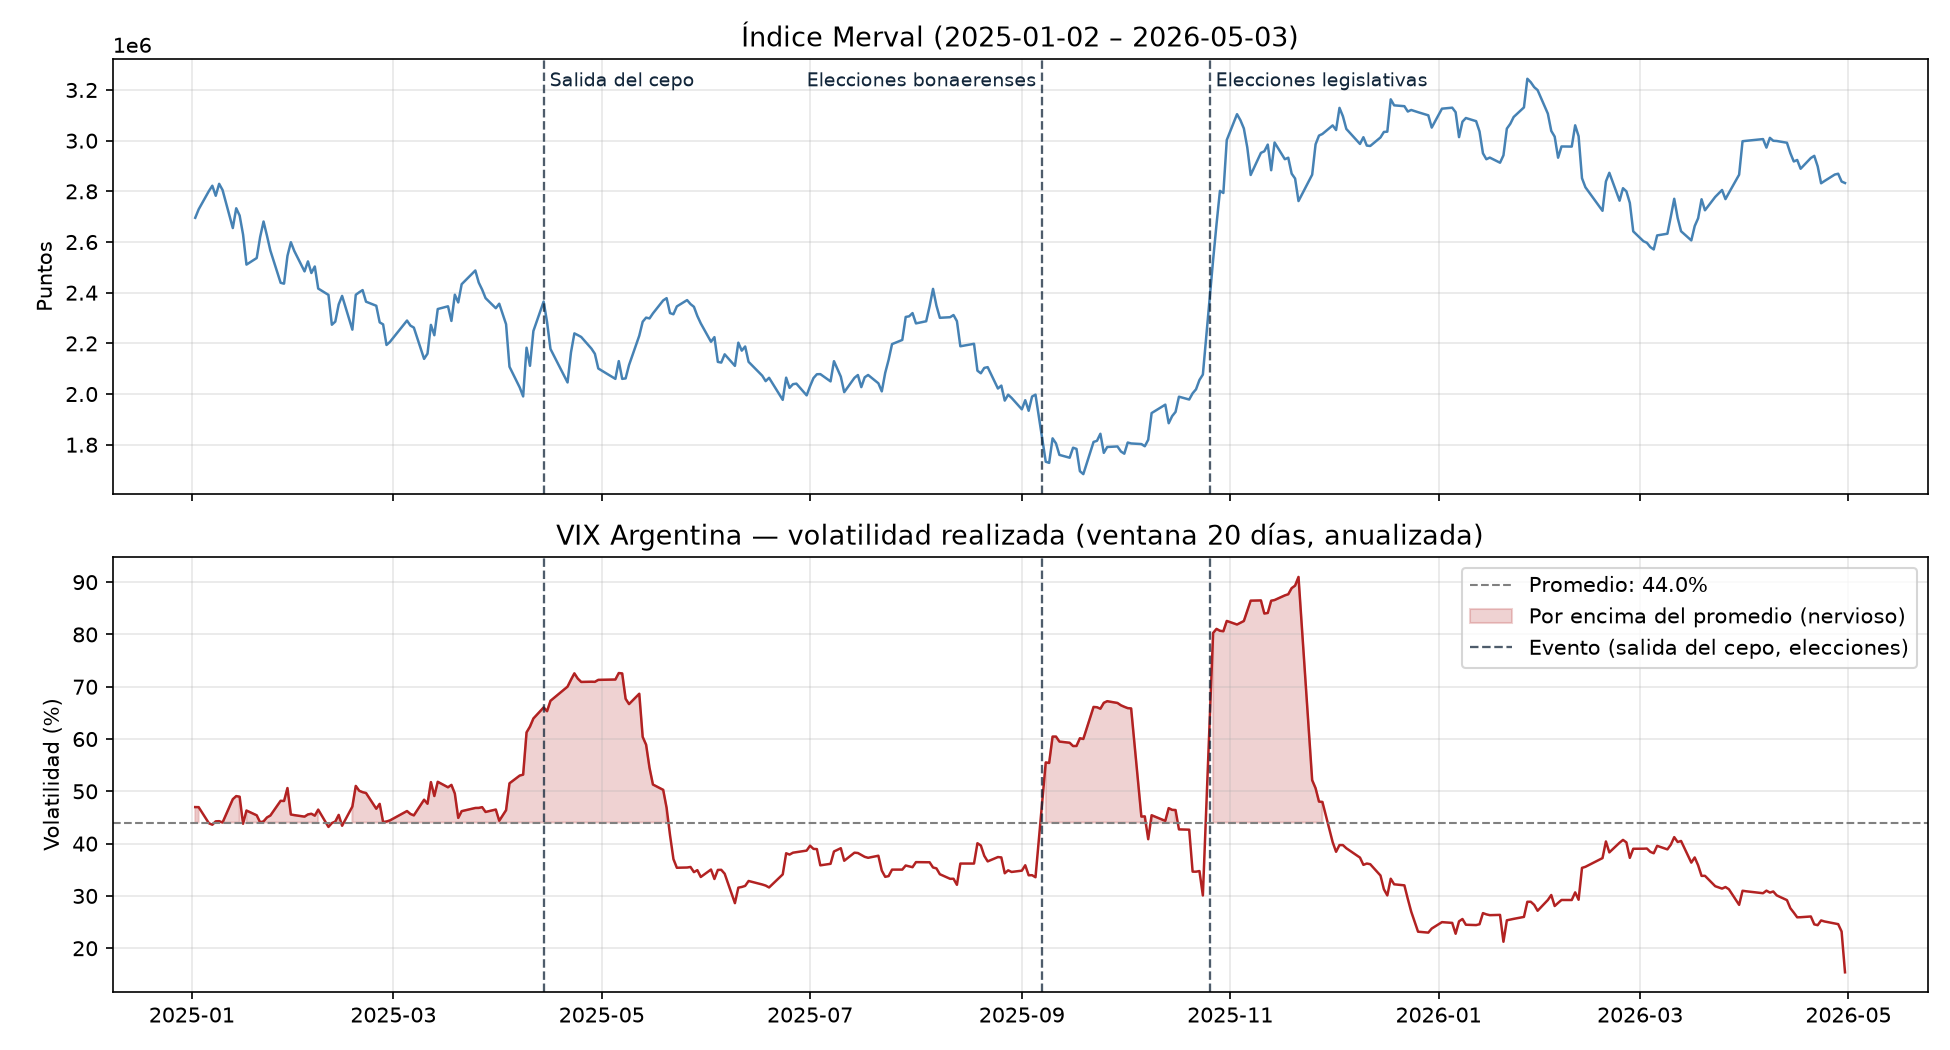
\includegraphics[width=0.88\linewidth]{vix_arg_reducida.png}
\caption{S\&P~Merval en pesos (arriba) y VIX argentino (abajo), del 2/1/2025 al 30/4/2026.
El sombreado marca los días por encima del promedio; las líneas punteadas, la salida del cepo
(14/04/2025) y las elecciones bonaerenses (07/09/2025) y legislativas (26/10/2025). Fuente:
elaboración propia con datos de Yahoo Finance (\carpeta{Lado Bursatil/03_vix_argentino}).}
\label{fig:vix}
\end{figure}

Hay una regla de lectura que conviene tener presente. Como el VIX argentino es un desvío de 20
ruedas, un único día extremo queda dentro del cálculo durante exactamente 20 ruedas: el índice
salta el día del shock y cae de golpe 20 ruedas después, aunque ese día el mercado no haga nada
especial. Las subidas bruscas marcan el día del shock; las bajadas bruscas, que el shock cumplió
20 ruedas. Por ejemplo, el VIX pasó de 91,0\% el 21/11/2025 a 52,1\% en la rueda siguiente,
cuando salió de la ventana la suba del 27/10. Este artefacto de las medias móviles con pesos
iguales está descrito en la literatura \citep{papaioannou2014}.

% ---------------------------------------------------------------------
\section{Cómo reacciona a los eventos}

El período tuvo tres episodios de volatilidad alta, todos disparados por un hecho puntual
(tabla~\ref{tab:episodios}).

\begin{table}[H]
\centering\small
\begin{tabularx}{\linewidth}{@{}L{3.1cm}C{1.1cm}L{2.6cm}L{2.2cm}Y@{}}
\toprule
\textbf{Período} & \textbf{Ruedas} & \textbf{Pico del VIX} & \textbf{Disparador} & \textbf{Contexto} \\
\midrule
09/04 al 14/05/2025 & 22 & 72,6\% (06/05) & 09/04: +9,7\% & Aranceles de EE.\,UU.; incluye la salida del cepo (14/04) \\
08/09 al 03/10/2025 & 20 & 67,2\% (26/09) & 08/09: $-$13,3\% & Día hábil siguiente a las elecciones bonaerenses (07/09) \\
27/10 al 21/11/2025 & 20 & 91,0\% (21/11) & 27/10: +21,8\% & Día hábil siguiente a las legislativas nacionales (26/10) \\
\bottomrule
\end{tabularx}
\caption{Episodios con el VIX argentino por encima de 55\%. Fuente: elaboración propia
(\carpeta{Lado Bursatil/03_vix_argentino}).}
\label{tab:episodios}
\end{table}

\textbf{La salida del cepo.} El primer episodio es el único que se construye de a poco. A
comienzos de abril de 2025, con la turbulencia global por los aranceles de Estados Unidos, el
índice cayó varios días seguidos y el VIX subió de 46\% a 53\%. El 09/04, el día de la pausa
de los aranceles, el Merval rebotó 9,7\% y el VIX pasó a 61\%. La salida del cepo cambiario, el
lunes 14/04, llegó con el mercado ya alterado: ese día el índice subió 5,2\% y el VIX llegó a
66\%. El pico del episodio (72,6\%) se alcanzó el 06/05, después de un mes de movimientos
grandes en las dos direcciones.

\textbf{Las elecciones.} Los otros dos episodios son lo contrario: un salto de un día. El
viernes anterior a las elecciones bonaerenses el VIX estaba en 33,6\%; el lunes 08/09, con una
caída de 13,3\% del índice, pasó a 55,5\% en una sola rueda. Antes de las legislativas
nacionales estaba en 30,1\%; el lunes 27/10, con la suba de 21,8\%, saltó a 80,3\%. El máximo de
toda la serie no vino entonces de una caída sino de una suba. Los dos episodios duran
exactamente 20 ruedas: son, casi en su totalidad, el eco de un único día. Dentro del primero cae
además el anuncio de apoyo financiero del Tesoro de Estados Unidos (24/09), con el VIX ya
cerca de 66\%.

% ---------------------------------------------------------------------
\section{La volatilidad de cada acción}

Aplicado a cada acción, el mismo cálculo muestra que cada una sola es más nerviosa que el
índice, que diversifica: su volatilidad promedio fue de 55,1\%, contra 44,0\% del VIX
(figura~\ref{fig:ranking}). La más calma fue Mirgor (36,2\%) y la más volátil, Celulosa
Argentina (104,6\%); por sector, Real Estate fue el más calmo (42,5\%) y Utilities el más volátil
(60,5\%). Se buscaron además \textit{picos propios}: tramos en que una acción está muy alterada
con el mercado tranquilo. De 19 tramos, 12 eran el eco de 20 ruedas del VIX; quedan 7 genuinos,
en CELU, SAMI, GARO y RIGO.

\begin{figure}[H]
\centering
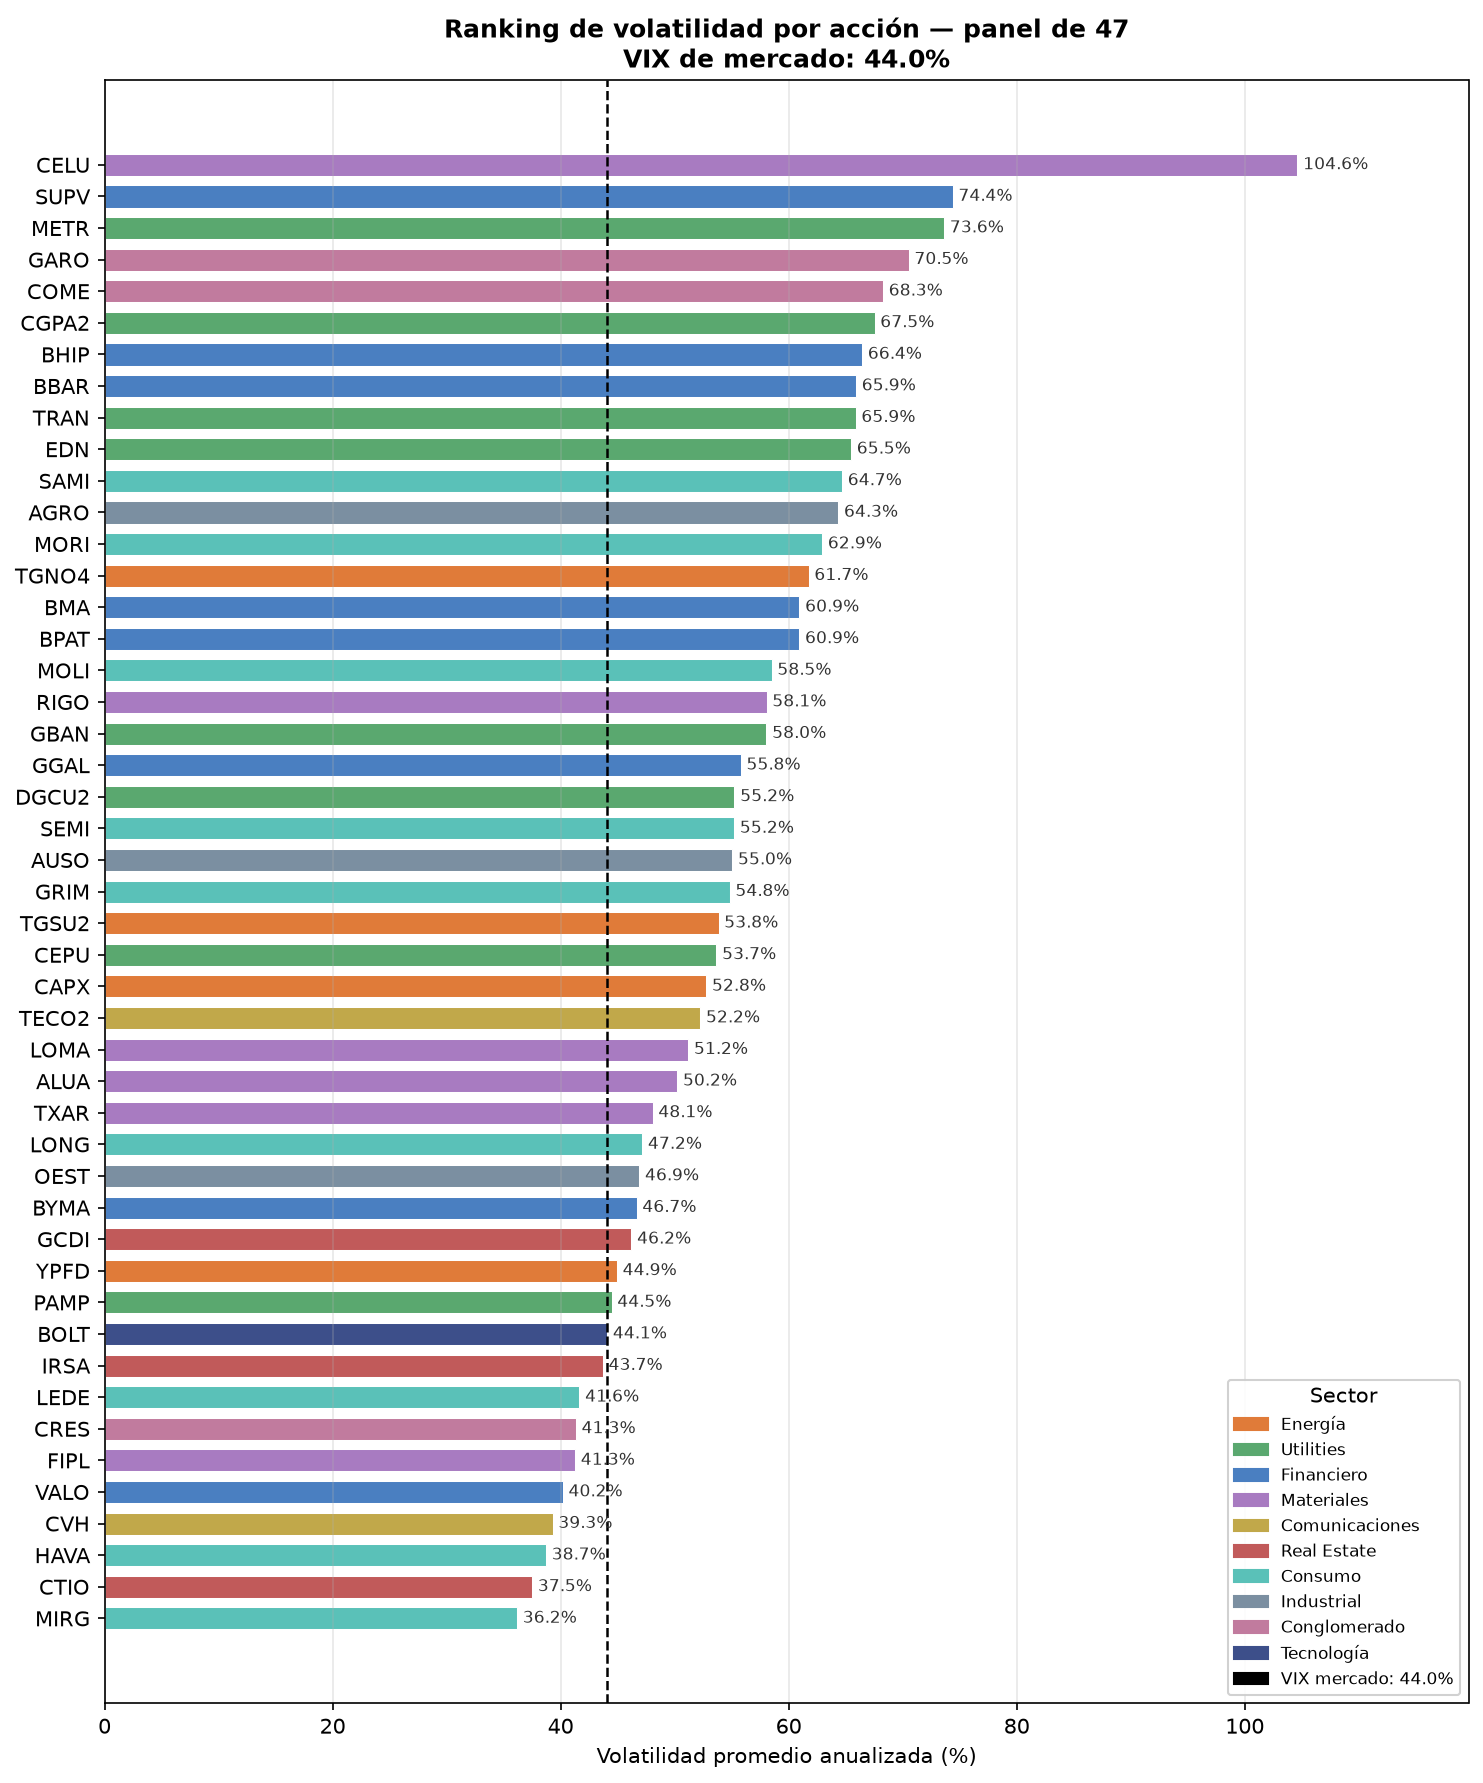
\includegraphics[width=0.48\linewidth]{ranking_volatilidad.png}
\caption{Volatilidad promedio de las 47 acciones, coloreada por sector, con el VIX argentino
como referencia (2/1/2025 al 30/4/2026). Fuente: elaboración propia
(\carpeta{Lado Bursatil/05_volatilidad_ranking}).}
\label{fig:ranking}
\end{figure}

El VIX argentino cumple su función de instrumento: identifica sin ambigüedad los días de shock
del período y los ordena por tamaño. Su límite es que es simétrico —sube igual con una suba que
con una caída, mientras que en el S\&P~Merval las caídas pesan más \citep{otuki2008}— y que
hereda el eco de las 20 ruedas, que también afecta a las fechas de los regímenes.

% ---------------------------------------------------------------------
\section{¿Hay familias de acciones? Clustering}
\label{sec:clustering}

Si existieran grupos de acciones que reaccionan de forma parecida, las noticias podrían
analizarse por familia, con más señal y menos ruido. El clustering agrupa elementos parecidos sin
etiquetas previas, usando como distancia entre dos acciones $1-\rho$, con $\rho$ la correlación de
sus retornos \citep{mantegna1999}. Se probaron tres algoritmos (K-Means, jerárquico y árbol de
expansión mínima), tres representaciones (retornos, log-volumen y 13 características como
volatilidad, asimetría y beta) y dos ventanas: 18 combinaciones, evaluadas con el índice de
silueta \citep{rousseeuw1987}. Casi todas las mejores aíslan una o dos acciones contra el resto;
la única que forma un grupo real es K-Means con las 13 características a tres años: 8 acciones,
con silueta 0,406.

Ese grupo no se explica por la volatilidad sino por la \textbf{liquidez}: sus acciones tienen
volumen irregular y baja correlación con el panel, porque los días sin operaciones repiten el
precio y bajan artificialmente la correlación \citep{nanyonga2025,lesmond1999}. Sacando las
cuatro con más días sin operar (GCDI, RIGO, GRIM y GARO), la silueta cae a 0,219 y el grupo se
deshace. No hay, entonces, familias de comportamiento: por eso el análisis con noticias se hizo
acción por acción y por sector, y esas cuatro acciones se leen con cautela, porque un precio
atrasado puede parecer una reacción con retraso \citep{lomackinlay1990}.

% =====================================================================
\chapter{Cuarto instrumento: los regímenes de mercado}
\chaptermark{Los regímenes de mercado}
\label{cap:hmm}

El VIX argentino dice cuánta tensión hay cada día, pero se mueve de forma muy dispareja: hay
tramos largos de calma y episodios cortos y violentos de estrés. Para trabajar con esa
alternancia hace falta una clasificación de los días según el estado del mercado. El cuarto
instrumento la produce con un modelo oculto de Markov: un modelo que supone que el mercado
pasa por unos pocos estados que no se observan directamente, y que los infiere de la
volatilidad.

% ---------------------------------------------------------------------
\section{El modelo}

Un modelo de cambio de régimen de Markov supone que la serie —aquí, el VIX argentino— tiene una
media y una varianza distintas en cada uno de $k$ estados ocultos, y que el mercado pasa de un
estado a otro según una matriz de probabilidades de transición
\citep{hamilton1989,kim1994}: la probabilidad de estar en un régimen mañana depende solo del
régimen de hoy. En la literatura de mercados se lo suele llamar HMM \citep{rabiner1989}. Se
estimó con \texttt{MarkovRegression} de \texttt{statsmodels}, con media y varianza propias de
cada régimen, sobre las 323 ruedas del VIX argentino.

A cada día se le asigna el régimen de mayor probabilidad \textit{suavizada}, que usa toda la
serie. Se guarda también la versión \textit{filtrada}, que solo usa la información disponible
hasta ese día y es la adecuada si el régimen se usa para pronosticar \citep{majumder2023}. Las
dos coinciden en el 98,5\% de los días.

% ---------------------------------------------------------------------
\section{¿Cuántos regímenes?}

El número de regímenes no se fijó a mano: se ajustó el modelo para $k=2$ a 6 y se comparó el
criterio bayesiano de información \citep[BIC;][]{schwarz1978}, que premia el ajuste y penaliza
los parámetros de más. Hubo que agregar una regla: descartar los ajustes que no convergen o que
crean un régimen de menos de cinco días. Un régimen de un solo día tiene varianza casi cero, su
verosimilitud se dispara y el BIC mejora de forma artificial: es una falla conocida de los
modelos de mezcla, no un estado real del mercado (tabla~\ref{tab:bic}).

\begin{table}[H]
\centering\small
\begin{tabularx}{\linewidth}{@{}cccccY@{}}
\toprule
$k$ & \textbf{BIC} & \textbf{Convergió} & \textbf{Régimen más chico} & \textbf{Válido} & \textbf{Qué pasa} \\
\midrule
2 & 2.202,9 & No & 1 día & No & Depende del arranque aleatorio \\
\textbf{3} & \textbf{2.119,4} & \textbf{Sí} & \textbf{65 días} & \textbf{Sí} & \textbf{Elegido; idéntico con 10 semillas} \\
4 & 2.152,0 & No & 1 día & No & Los mismos 3 regímenes más un día suelto (01/12/2025) \\
5 & 2.161,4 & No & 1 día & No & Un estado clavado en el mínimo de la serie \\
6 & 2.185,2 & No & 1 día & No & Ídem \\
\bottomrule
\end{tabularx}
\caption{Selección del número de regímenes. Fuente: elaboración propia
(\carpeta{Lado Bursatil/06_hmm_regimen_mercado}).}
\label{tab:bic}
\end{table}

Con $k=3$ el BIC es el menor entre los ajustes válidos, y el resultado es el mismo con diez
semillas distintas: no depende del punto de partida (figura~\ref{fig:bic}).

\begin{figure}[H]
\centering
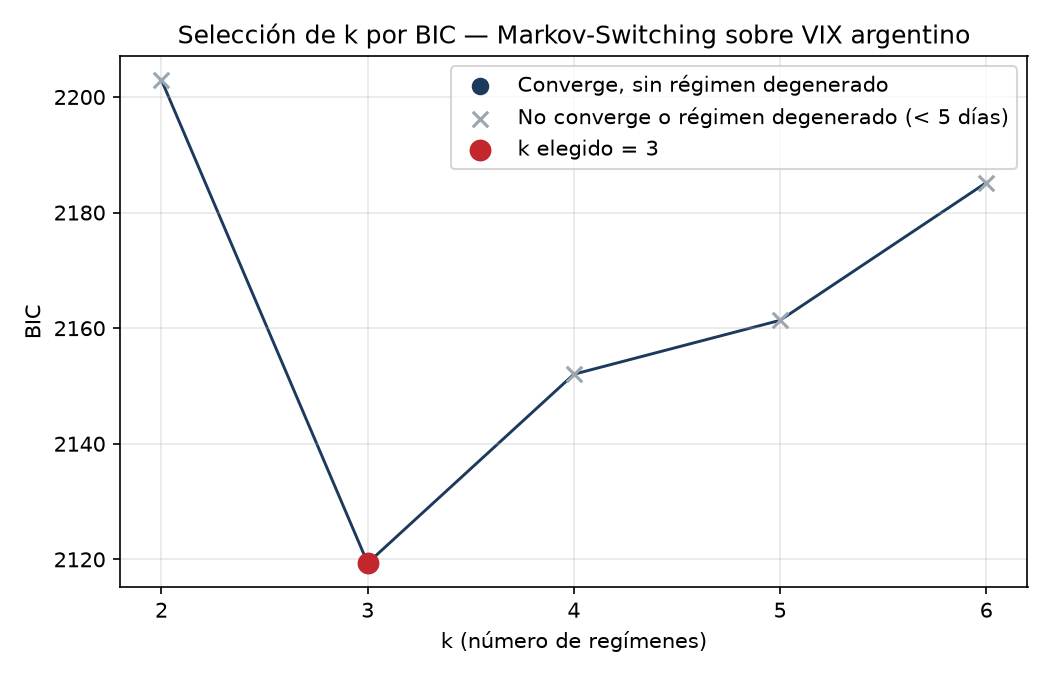
\includegraphics[width=0.5\linewidth]{bic_curva.png}
\caption{BIC según la cantidad de regímenes. Fuente: elaboración propia
(\carpeta{Lado Bursatil/06_hmm_regimen_mercado}).}
\label{fig:bic}
\end{figure}

% ---------------------------------------------------------------------
\section{Los tres regímenes}

La tabla~\ref{tab:regimenes} describe los tres regímenes, que se nombraron por su nivel de
volatilidad.

\begin{table}[H]
\centering\small
\begin{tabular}{@{}lrrrr@{}}
\toprule
\textbf{Régimen} & \textbf{VIX promedio} & \textbf{Retorno diario promedio} & \textbf{Días} & \textbf{\% del período} \\
\midrule
Calmo & 33,0\% & $-$0,074\% & 177 & 54,8 \\
Moderado & 46,6\% & 0,053\% & 81 & 25,1 \\
Tenso & 70,8\% & 0,518\% & 65 & 20,1 \\
\bottomrule
\end{tabular}
\caption{Regímenes del mercado entre el 2/1/2025 y el 30/4/2026 (323 ruedas). Fuente:
elaboración propia (\carpeta{Lado Bursatil/06_hmm_regimen_mercado}).}
\label{tab:regimenes}
\end{table}

Los regímenes son muy persistentes: la probabilidad de seguir en el mismo régimen al día
siguiente es de 98,0\% en Calmo, 95,8\% en Moderado y 95,1\% en Tenso
(tabla~\ref{tab:transicion}). Más interesante es cómo se pasa de uno a otro. La salida del
estrés es gradual: de Tenso nunca se volvió directo a Calmo, sino siempre a través de Moderado.
La entrada, en cambio, no: las dos veces que el mercado salió de Calmo saltó directo a Tenso,
y las dos fueron el día hábil siguiente a una elección (08/09 y 27/10/2025). El régimen Tenso
tiene el retorno promedio más alto porque incluye la fuerte suba posterior a las legislativas:
la tensión no es lo mismo que la caída.

\begin{table}[H]
\centering\small
\begin{tabular}{@{}lccc@{}}
\toprule
\textbf{De \flecha{} a} & \textbf{Calmo} & \textbf{Moderado} & \textbf{Tenso} \\
\midrule
Calmo & 98,0\% & 0,0\% & 2,0\% \\
Moderado & 4,2\% & 95,8\% & 0,0\% \\
Tenso & 0,0\% & 4,9\% & 95,1\% \\
\bottomrule
\end{tabular}
\caption{Probabilidad de pasar de un régimen (fila) a otro (columna) de una rueda a la
siguiente. Fuente: elaboración propia (\carpeta{Lado Bursatil/06_hmm_regimen_mercado}).}
\label{tab:transicion}
\end{table}

La figura~\ref{fig:hmm} muestra la secuencia completa. El período empieza en Moderado, pasa a
Tenso el 07/04/2025 con los aranceles y la salida del cepo, y se calma desde fines de mayo. Los
dos episodios electorales son tramos Tenso de exactamente 20 ruedas, del 08/09 al 03/10 y del
27/10 al 21/11: el modelo hereda el eco del VIX (capítulo~\ref{cap:vix}). Desde el 01/12/2025
hasta el final de la ventana el mercado queda en Calmo, durante 100 ruedas seguidas.

\begin{figure}[H]
\centering
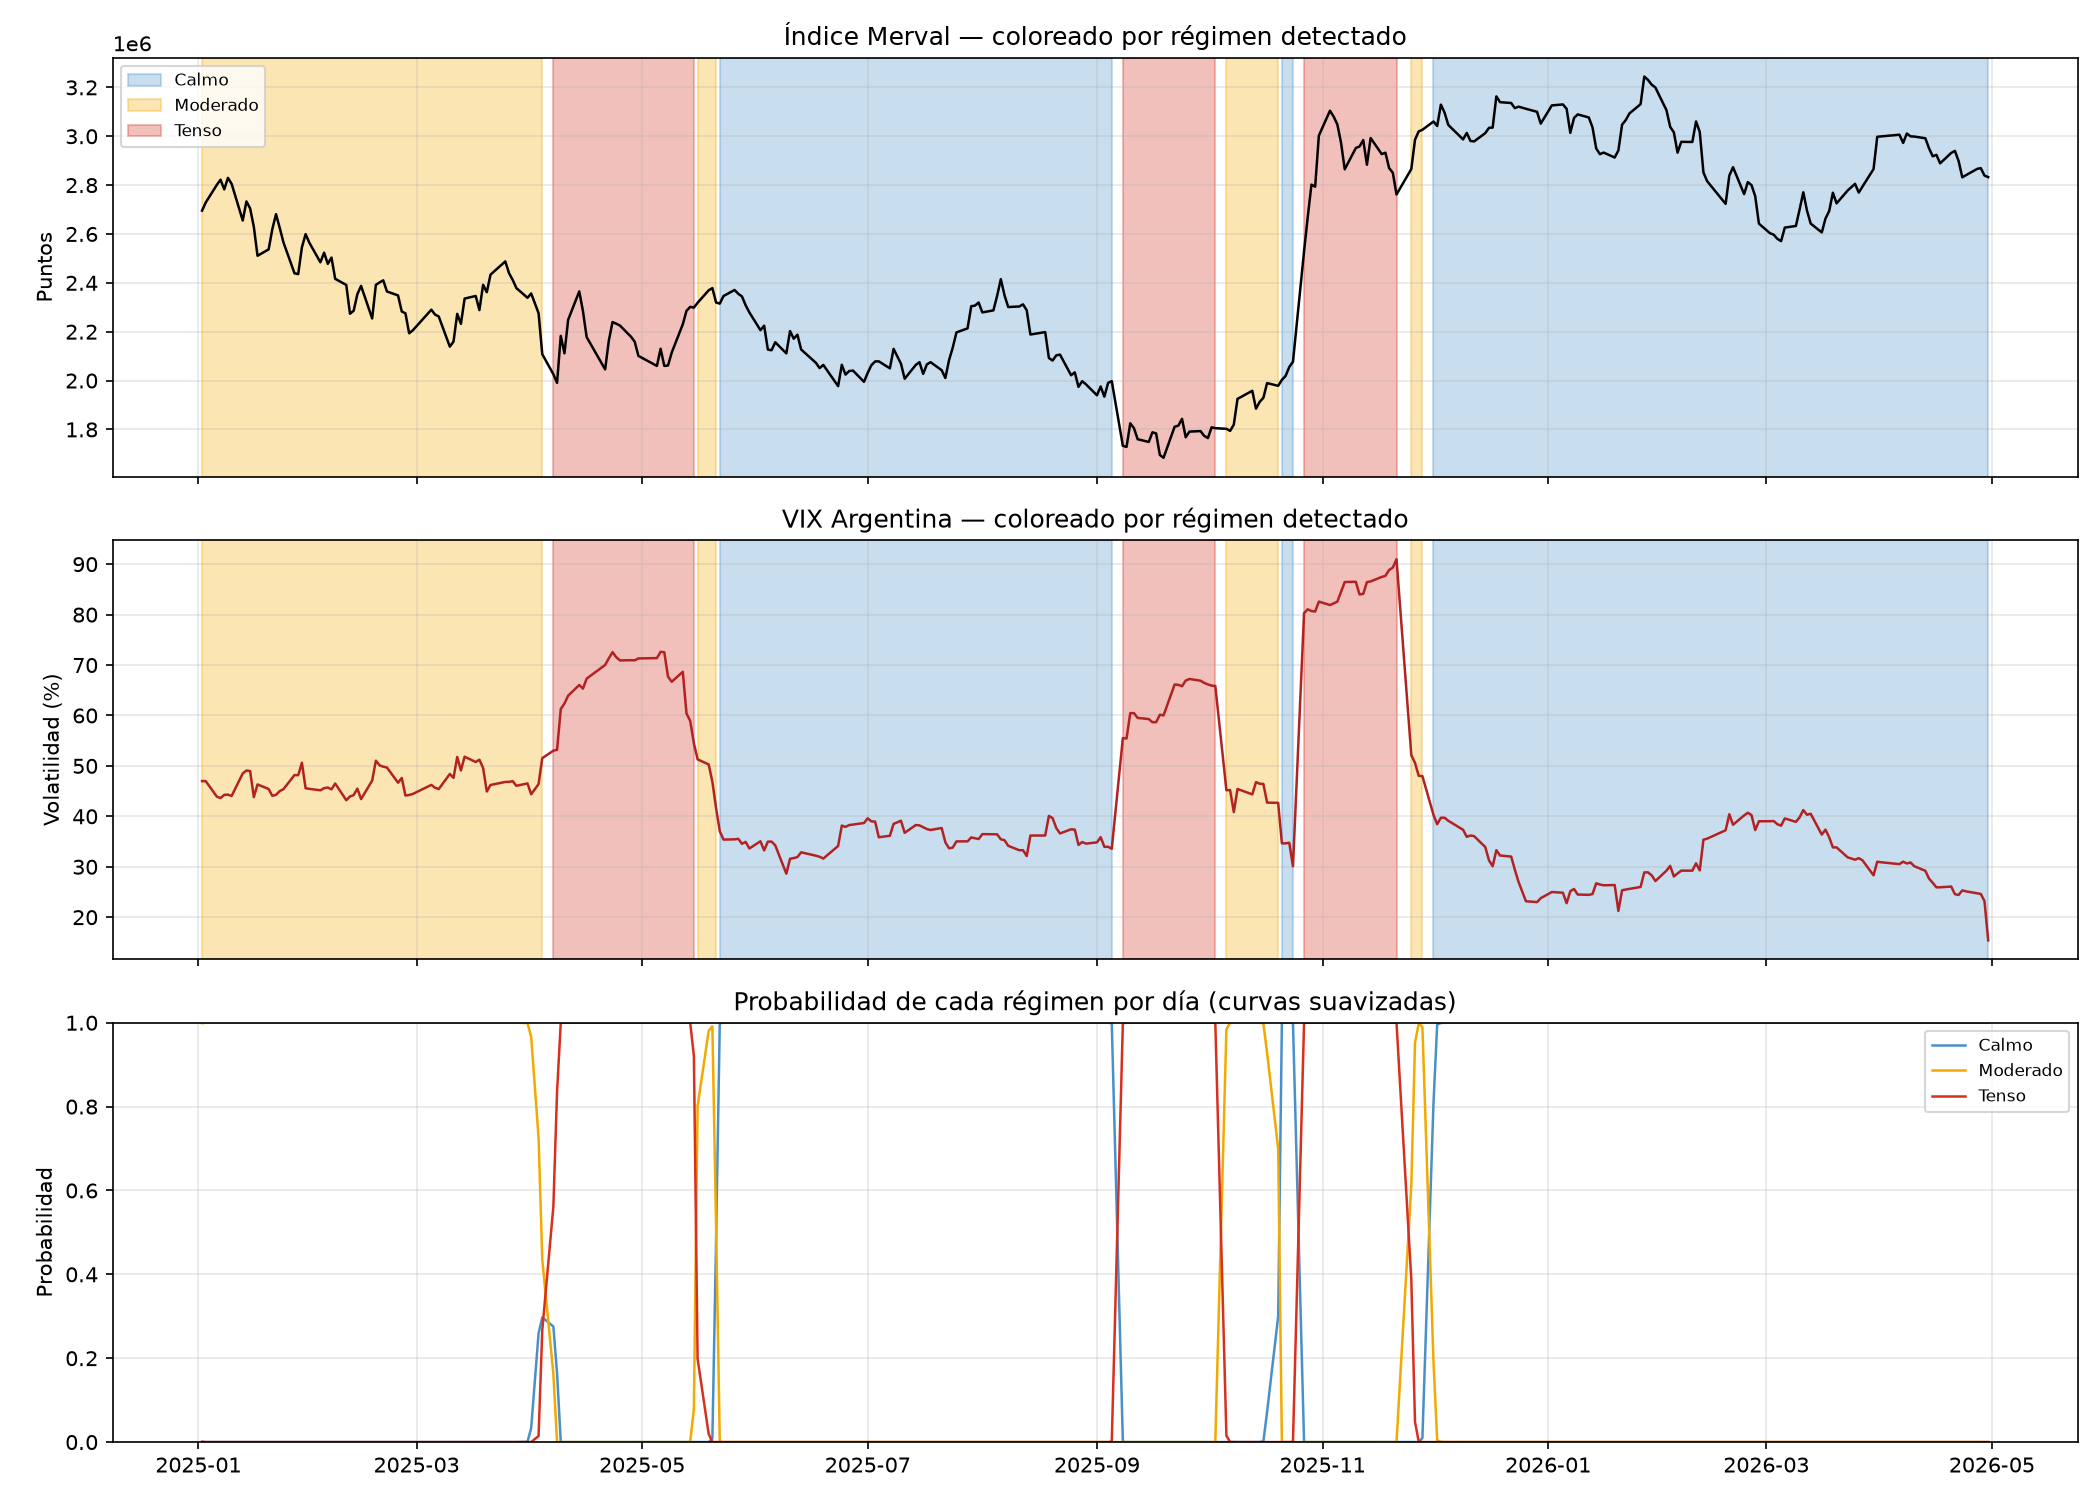
\includegraphics[width=0.8\linewidth]{hmm_regimen_mercado.png}
\caption{S\&P~Merval y VIX argentino coloreados por régimen, y probabilidad suavizada de cada
régimen por día. Fuente: elaboración propia (\carpeta{Lado Bursatil/06_hmm_regimen_mercado}).}
\label{fig:hmm}
\end{figure}

\textbf{Para qué sirve en la tesina.} El régimen es la variable de contexto con la que se
pregunta si la relación entre noticias y precios cambia según el estado del mercado
\citep{garcia2013}. En la ventana común con las noticias (244 ruedas) hay 177 ruedas Calmo, 18
Moderado y 49 Tenso; como Moderado queda con muy pocas ruedas, el análisis por régimen del
capítulo~\ref{cap:var} compara Calmo contra Tenso.

% =====================================================================
\chapter{El experimento: VAR y causalidad de Granger}
\chaptermark{VAR y causalidad de Granger}
\label{cap:var}

Con los cuatro instrumentos construidos, la pregunta de la tesina se puede contrastar: ¿el tono
de las noticias anticipa el precio y el volumen de las acciones, o es al revés? Este capítulo
une los dos lados, prepara las series, presenta el modelo y sus resultados, y resume las pruebas
complementarias y la robustez.

% ---------------------------------------------------------------------
\section{La unión de los instrumentos}
\label{sec:union}

Los dos lados se unieron en la ventana en la que ambos tienen datos: 244 ruedas, del
05/05/2025 al 30/04/2026. Todo quedó en dos tablas: una por rueda (el mercado) y otra por acción
y rueda (11.468 filas). Del lado de las noticias, las variables son el tono anormal, la atención
anormal y el tono propio de las 17 empresas (capítulo~\ref{cap:finbeto}). Del lado del mercado,
el retorno diario del S\&P~Merval y de cada acción, y el \textit{volumen anormal}:
$\log(1+\text{volumen}_t)$ menos su promedio en las 20 ruedas previas, para que sea comparable
entre acciones y no crezca con la inflación. El régimen del capítulo~\ref{cap:hmm} marca cada
rueda, y se marcaron aparte los dos días electorales, su eco y abril de 2026. En la ventana, el
retorno del S\&P~Merval promedió 0,16\% diario con un desvío de 2,79\%, y sus extremos son los
dos días electorales ($-13{,}25\%$ y $+21{,}77\%$).

\textbf{Estacionariedad.} Un VAR necesita series estacionarias, que oscilen alrededor de un nivel
estable: si no, dos variables con tendencia parecen relacionadas aunque no lo estén. Se usaron dos
pruebas que preguntan al revés: la ADF \citep{dickey1979}, cuya hipótesis nula es que la serie no
es estacionaria, y la KPSS \citep{kpss1992}, cuya nula es que sí lo es. En el lado bursátil, con
tres años de datos, 46 de los 47 precios no son estacionarios y los 47 retornos sí: por eso los
modelos usan retornos y no precios \citep{zablotsky2002}. En la ventana de la unión se probaron
156 series: retornos, volúmenes anormales, atención y tono propio son estables. El tono en nivel
dio \textit{inconcluso}, porque cambia en ciclos de meses (promedio trimestral de $+7{,}5$, $+0{,}5$,
$+7{,}6$, $+3{,}7$ y $-2{,}9$), un rasgo conocido de las series de tono \citep{correarocha2026}; por
eso el modelo usa el \textit{tono anormal}, que es estable sin discusión. El VIX también dio
inconcluso y entra a los modelos solo a través del régimen.

% ---------------------------------------------------------------------
\section{El modelo}

Un VAR con $p$ rezagos explica el vector de variables de hoy, $y_t$, con sus valores de las $p$
ruedas anteriores:
\begin{equation}
y_t = c + A_1\, y_{t-1} + A_2\, y_{t-2} + \dots + A_p\, y_{t-p} + \varepsilon_t .
\end{equation}
Cuántas ruedas hacia atrás mira el modelo (los \textit{rezagos}) se eligió automáticamente entre
1 y 5 con el criterio de Akaike \citep{lutkepohl2005}, que busca el equilibrio entre ajustar bien
los datos y no complicar el modelo de más.

La prueba de Granger \citep{granger1969} responde una pregunta concreta: ¿conocer el tono de las
ruedas anteriores mejora la predicción del retorno de hoy, más allá de lo que ya predicen los
retornos anteriores? Si la mejora es estadísticamente significativa, el tono \textit{anticipa} al
retorno. La misma pregunta se hace al revés, para ver si el retorno anticipa al tono. La función
de impulso-respuesta, además, muestra cómo responde cada variable, rueda a rueda, a un golpe en
otra.

Se usaron 224 ruedas, del 02/06/2025 al 30/04/2026: las primeras 20 de la ventana quedan afuera
porque no tienen 20 ruedas previas con las que calcular el tono anormal. La prueba se repitió en
cinco niveles —el mercado, cada una de las 47 empresas, las 17 con tono propio, los 10 sectores y
los regímenes—, en las dos direcciones y con precio y volumen: 304 pruebas en total. Todos los
modelos resultaron estables, es decir, el efecto de un golpe se apaga con el tiempo en lugar de
crecer.

\textbf{Pruebas múltiples.} Con tantas pruebas, algunas salen significativas por azar: con 100
pruebas al 5\%, se esperan unas 5 aunque no haya ningún efecto \citep{harvey2016}. Por eso los
p-valores se corrigieron con Benjamini-Hochberg \citep{bh1995}, que los «encarece» para no
confundir casualidades con efectos; en todas las tablas, «significativo» quiere decir $p$
\textit{corregido} menor a 0,05. Como control, la prueba por empresa se repitió con el tono
mezclado al azar, lo que rompe cualquier relación real: el test debería indicar un efecto, por
error, en alrededor del 5\% de las pruebas, y dio 6,9\%. El método no encuentra efectos donde no
los hay.

% ---------------------------------------------------------------------
\section{¿Quién anticipa a quién?}
\label{sec:res-u6}

\subsection{El mercado}

De las ocho pruebas del VAR del mercado, una sola es significativa, y es fuerte: el retorno del
S\&P~Merval anticipa el tono anormal de las noticias ($p$ corregido 0,0003). Ninguna prueba en la
dirección de las noticias hacia el mercado llega a ser significativa (tabla~\ref{tab:u6-mercado}).

\begin{table}[H]
\centering\small
\begin{tabular}{@{}llccc@{}}
\toprule
\textbf{Prueba} & \textbf{Dirección} & \textbf{p} & \textbf{p corregido} & \textbf{Significativo} \\
\midrule
tono \flecha{} retorno & Noticias \flecha{} mercado & 0,2119 & 0,4238 & No \\
retorno \flecha{} tono & Mercado \flecha{} noticias & $<$0,0001 & 0,0003 & \textbf{Sí} \\
tono \flecha{} volumen & Noticias \flecha{} mercado & 0,0632 & 0,2528 & No \\
volumen \flecha{} tono & Mercado \flecha{} noticias & 0,3617 & 0,4823 & No \\
atención \flecha{} retorno & Noticias \flecha{} mercado & 0,9293 & 0,9293 & No \\
retorno \flecha{} atención & Mercado \flecha{} noticias & 0,1479 & 0,3944 & No \\
atención \flecha{} volumen & Noticias \flecha{} mercado & 0,3377 & 0,4823 & No \\
volumen \flecha{} atención & Mercado \flecha{} noticias & 0,5918 & 0,6764 & No \\
\bottomrule
\end{tabular}
\caption{Pruebas de causalidad de Granger en el VAR del mercado (224 ruedas). Tono: tono anormal
de las noticias de la rueda (tono menos el promedio de las 20 ruedas previas). Atención: cantidad
de notas comparada con lo habitual. Volumen: monto operado anormal. Fuente: elaboración propia
(\carpeta{Unión/06_var_granger}).}
\label{tab:u6-mercado}
\end{table}

La impulso-respuesta dimensiona el efecto (figura~\ref{fig:irf}). Un día en que el S\&P~Merval
sube un desvío (2,8\%), el tono anormal sube 1,84 puntos en la rueda siguiente y 1,23 en la
segunda, ambos distintos de cero; a la tercera ya no se distingue de cero. Como un desvío del
tono anormal son 6,0 puntos, la suba de la rueda siguiente es de un tercio de desvío. El tono y el
retorno de una misma rueda también se mueven juntos (correlación 0,19), pero con datos diarios no
se puede saber quién movió a quién dentro de la rueda. Desde la rueda siguiente, el efecto del
tono sobre el retorno ya no se distingue de cero.

\begin{figure}[H]
\centering
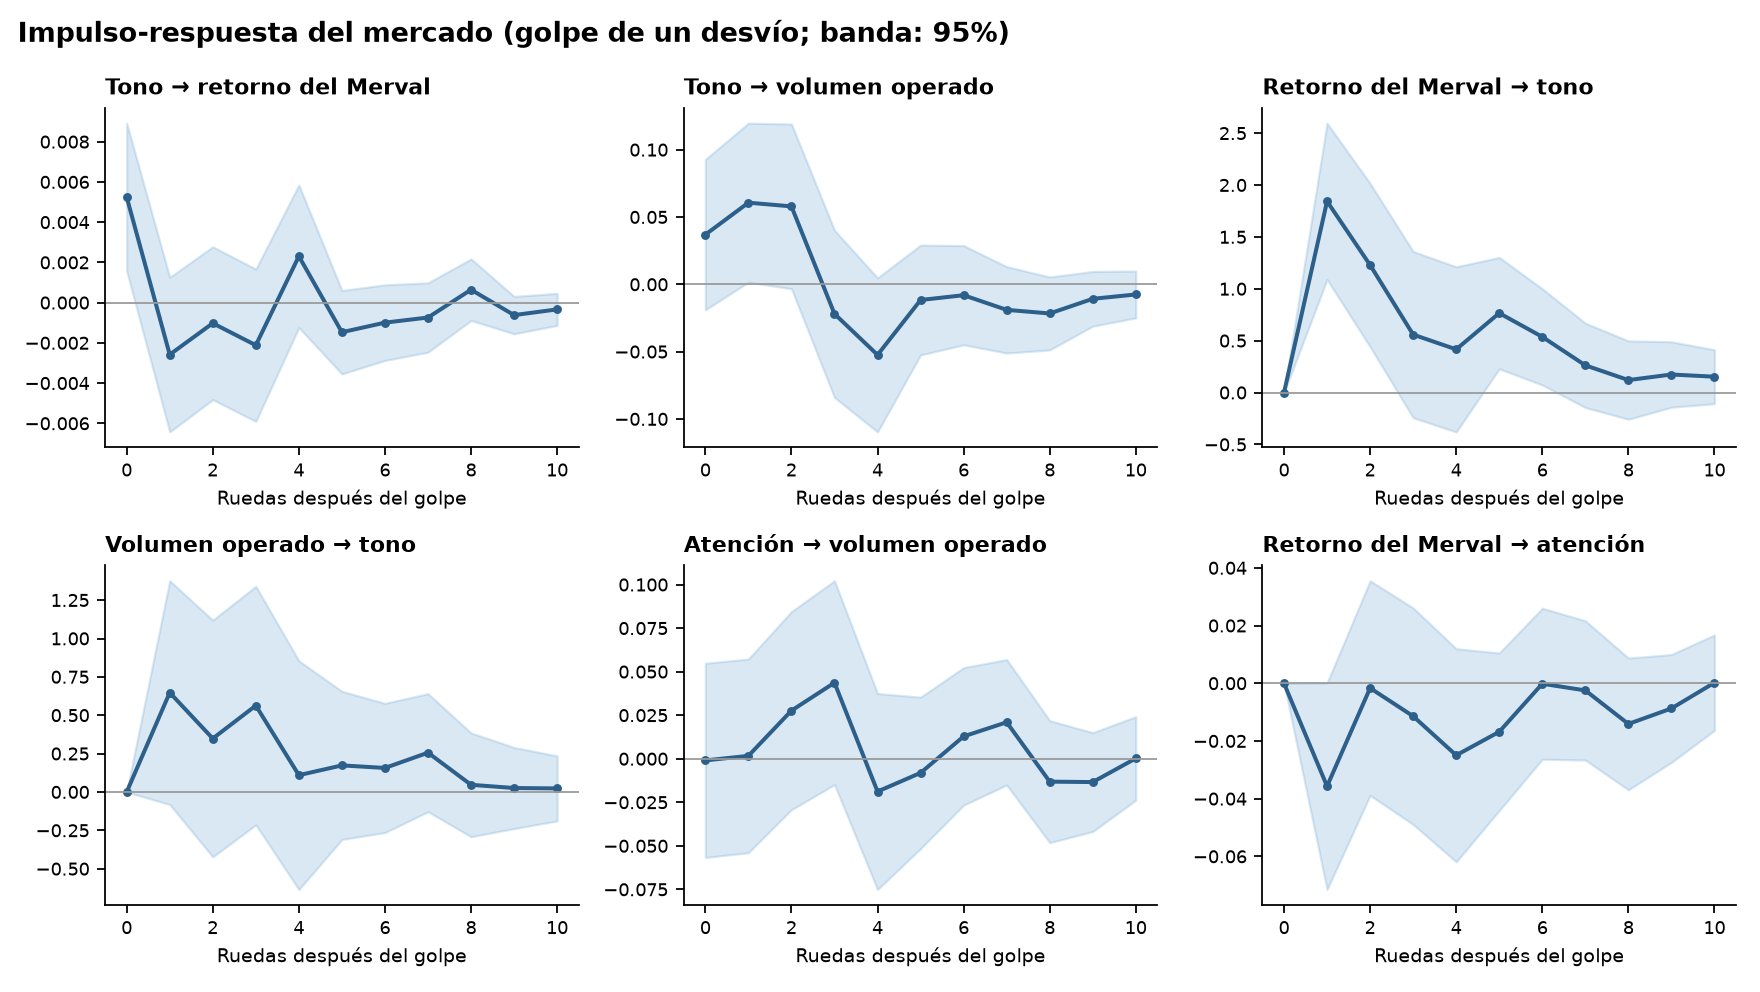
\includegraphics[width=0.8\linewidth]{u6_irf_mercado.png}
\caption{Funciones de impulso-respuesta del VAR del mercado ante un golpe de un desvío, con
banda del 95\%. Si la banda no toca el cero, la respuesta es distinta de cero. Fuente:
elaboración propia (\carpeta{Unión/06_var_granger}).}
\label{fig:irf}
\end{figure}

\subsection{Las empresas}

El retorno de casi todas las empresas anticipa el tono de las noticias: 39 de 47, todas con
signo positivo (tabla~\ref{tab:u6-empresas}). En este nivel el tono es el del mercado, y los
retornos de las empresas se mueven con el índice, de modo que en buena parte es el mismo hallazgo
del mercado repetido. En la dirección contraria, 7 de 94 pruebas dan $p<0{,}05$ sin corregir,
menos de las 9,4 que se esperarían por azar; después de la corrección quedan dos, sin un patrón.

\begin{table}[H]
\centering\small
\begin{tabular}{@{}lcccc@{}}
\toprule
\textbf{Prueba} & \textbf{Pruebas} & \textbf{$p<0{,}05$ sin corregir} & \textbf{Significativas} & \textbf{Signo} \\
\midrule
\multicolumn{5}{@{}l}{\textit{47 empresas, con el tono del mercado}} \\
tono \flecha{} retorno & 47 & 1 & 0 & — \\
tono \flecha{} volumen & 47 & 6 & 2 & 2 positivas \\
retorno \flecha{} tono & 47 & 43 & \textbf{39} & 39 positivas \\
volumen \flecha{} tono & 47 & 11 & 3 & 3 positivas \\
\midrule
\multicolumn{5}{@{}l}{\textit{17 empresas, con su tono propio}} \\
tono propio \flecha{} retorno & 17 & 0 & 0 & — \\
tono propio \flecha{} volumen & 17 & 2 & 1 & 1 positiva \\
retorno \flecha{} tono propio & 17 & 16 & \textbf{15} & 15 positivas \\
volumen \flecha{} tono propio & 17 & 1 & 0 & — \\
\bottomrule
\end{tabular}
\caption{Pruebas de Granger por empresa. «Significativas» cuenta las que siguen siéndolo
después de la corrección. Fuente: elaboración propia (\carpeta{Unión/06_var_granger}).}
\label{tab:u6-empresas}
\end{table}

La prueba más exigente es la del tono propio, que descuenta el clima general de las noticias. En
15 de las 17 empresas, cuando la acción sube, en las ruedas siguientes se habla de ella mejor que
del resto del mercado: BBAR, BMA, BYMA, CEPU, CRES, EDN, GGAL, IRSA, LOMA, METR, SUPV, TGSU2,
TRAN, TXAR e YPFD (no aparece en ALUA ni en PAMP). Es el resultado más fuerte de la tesina,
porque es específico de cada empresa (figura~\ref{fig:u6-empresas}). En la dirección contraria
queda una sola prueba significativa (IRSA, tono propio \flecha{} volumen), aislada.

\begin{figure}[H]
\centering
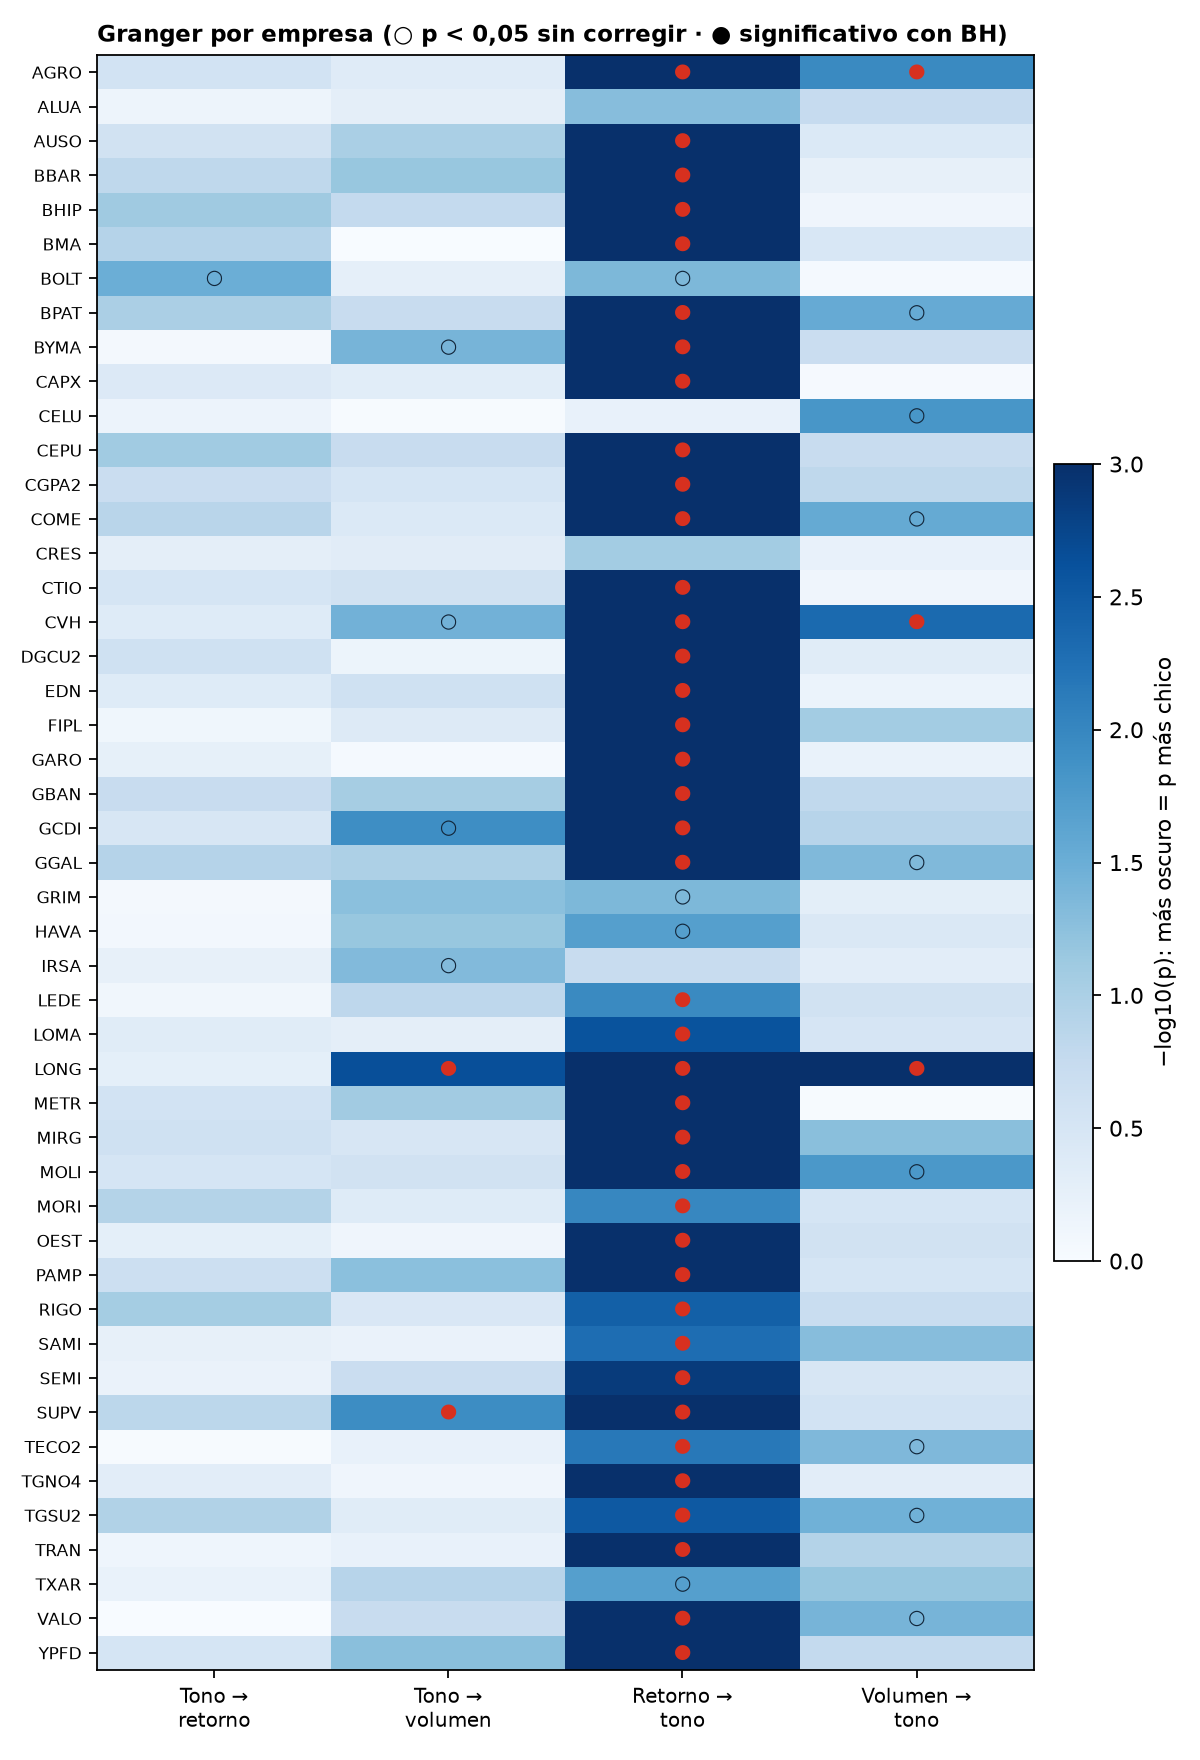
\includegraphics[width=0.42\linewidth]{u6_empresas.png}
\caption{Pruebas de Granger por empresa. Cada fila es una empresa y cada columna una prueba;
más oscuro, $p$ más chico; $\circ$ $p<0{,}05$ sin corregir; $\bullet$ significativo después
de la corrección. Fuente: elaboración propia (\carpeta{Unión/06_var_granger}).}
\label{fig:u6-empresas}
\end{figure}

\subsection{Los sectores y el régimen}

\textbf{Sectores.} Se repitió el VAR con el promedio de las acciones de cada uno de los diez
sectores. La dirección mercado \flecha{} noticias aparece en casi todos: en 9 de los 10, cuando el
sector sube, el tono de las ruedas siguientes es más positivo. La excepción es Tecnología, que
tiene una sola acción (BOLT). La dirección contraria aparece una sola vez: en Conglomerado el tono
anticipa el volumen, pero con signo negativo (más tono, menos volumen), un resultado aislado.

\textbf{Balance de todos los niveles.} Sumando mercado, empresas, tono propio y sectores, se
hicieron 152 pruebas en la dirección noticias \flecha{} mercado. Solo 4 son significativas, que es
lo que cabría esperar por azar con tantas pruebas, y no forman un patrón.

\textbf{Régimen.} La pregunta es si la relación cambia según el estado del mercado: la literatura
encuentra el efecto de las noticias sobre todo en los períodos de estrés \citep{garcia2013}. Con
los regímenes del capítulo~\ref{cap:hmm} se estimó un solo modelo con todas las ruedas y una marca
de día Tenso, para no pegar días que no son consecutivos; las 18 ruedas Moderado quedan afuera,
de modo que se comparan 166 días Calmo con 40 Tenso. Para cada prueba se pregunta tres cosas: si
hay efecto en los días Calmo, si hay efecto en los Tenso y si el efecto es distinto entre ambos.
La tabla~\ref{tab:u6-regimen} muestra los $p$ corregidos: un número chico indica que hay efecto, y
uno grande, que puede ser casualidad.

\begin{table}[H]
\centering\small
\begin{tabularx}{\linewidth}{@{}lcccY@{}}
\toprule
\textbf{Prueba} & \textbf{Días Calmo} & \textbf{Días Tenso} & \textbf{¿Cambia con el régimen?} & \textbf{Lectura} \\
\midrule
tono \flecha{} retorno & 0,42 & 0,92 & 0,95 & Nunca \\
tono \flecha{} volumen & 0,12 & 0,42 & 0,42 & Nunca \\
retorno \flecha{} tono & \textbf{0,007} & \textbf{0,007} & 0,81 & En los dos regímenes, igual \\
volumen \flecha{} tono & 0,60 & \textbf{0,008} & 0,12 & Solo en Tenso, sin diferencia significativa con Calmo \\
\bottomrule
\end{tabularx}
\caption{Pruebas de Granger según el régimen: $p$ corregido por Benjamini-Hochberg; en negrita,
menor a 0,05. «¿Cambia con el régimen?» prueba si el efecto es distinto en los días Tenso que en
los Calmo. Fuente: elaboración propia (\carpeta{Unión/06_var_granger}).}
\label{tab:u6-regimen}
\end{table}

La lectura es directa. \textbf{El tono no anticipa al mercado en ningún régimen}, ni siquiera en
los días de mayor estrés. \textbf{El retorno anticipa el tono en los dos regímenes y con la misma
fuerza}: los medios siguen al mercado tanto en calma como en tensión. El volumen anticipa el tono
solo en los días Tenso, pero la diferencia con los Calmo no llega a ser significativa: con 40 días
Tenso, los datos no alcanzan para afirmar que el régimen cambie la relación.

% ---------------------------------------------------------------------
\section{Dónde está el efecto: las notas de la misma noche}

La regla de las 17:00 manda las notas publicadas después del cierre a la rueda siguiente. Para
ver dónde está el efecto del retorno sobre el tono, se separaron las notas según la franja en que
se publicaron (tabla~\ref{tab:franjas}).

\begin{table}[H]
\centering\footnotesize
\begin{tabular}{@{}lrcc@{}}
\toprule
\textbf{Franja de publicación} & \textbf{Notas} & \textbf{Efecto de un desvío del retorno} & \textbf{p} \\
\midrule
Noche del día de la rueda (17 a 24 h) & 3.451 & \textbf{+4,77 puntos de tono} & $<$0,0001 \\
Día sin rueda & 2.142 & +3,11 & 0,1133 \\
Madrugada y mañana siguientes (antes de las 11) & 4.331 & +0,54 & 0,5142 \\
Sesión (11 a 17 h) & 4.001 & +1,26 & 0,1028 \\
\bottomrule
\end{tabular}
\caption{Relación entre el retorno de una rueda y el tono de las notas según la franja en que
se publicaron. Fuente: elaboración propia (\carpeta{Unión/08_robustez}).}
\label{tab:franjas}
\end{table}

El efecto está en las notas publicadas entre las 17:00 y la medianoche del día de la rueda: un
desvío del retorno sube su tono 4,8 puntos. En las notas de la madrugada y la mañana siguiente es
casi nulo. Por eso en el VAR aparece como «el retorno de hoy anticipa el tono de mañana»: después
del cierre, los medios cuentan cómo le fue al mercado y a cada empresa con un tono que acompaña la
suba o la baja, y no hay un arrastre que dure días.

% ---------------------------------------------------------------------
\section{Pruebas complementarias}
\label{sec:complementarias}

El VAR se complementó con tres pruebas (tabla~\ref{tab:complementarias}). La primera usa solo
las 8.069 notas publicadas con el mercado cerrado, que salen antes de cualquier operación de la
rueda: si su tono anticipa el salto de apertura, eso es noticias \flecha{} mercado sin ambigüedad
\citep{glasserman2025}. Las otras dos son estudios de eventos \citep{mackinlay1997}: alrededor
de las ruedas de tono extremo del mercado (16 eventos) y de cada empresa (88), con el retorno
normal estimado en las ruedas $[-25,-4]$ y el anormal medido antes, el día y después, contra
5.000 sorteos de fechas al azar; y alrededor de los shocks de cantidad con la definición del
plan ($z>2$ contra las 30 ruedas previas), medida por día de calendario porque la versión
original marcaba casi solo lunes. Dos de estas pruebas se especificaron por escrito antes de ver
los resultados.

\begin{table}[H]
\centering\footnotesize
\begin{tabularx}{\linewidth}{@{}L{3.3cm}YL{3.2cm}@{}}
\toprule
\textbf{Prueba} & \textbf{Resultado} & \textbf{Lectura} \\
\midrule
Notas con el mercado cerrado y retorno de apertura & Con notas de la noche más positivas el mercado abre algo más arriba (+0,18\% por desvío), pero no es significativo ($p=0{,}107$). Sin los dos días electorales, +0,06\% & El indicio se apoya en las elecciones: lo que movió la apertura fue el resultado, no el tono \\
Ruedas de tono extremo positivo (7 eventos) & El S\&P~Merval sube 2,01\% ese día (7 de 7; $p=0{,}018$ contra el azar) y ya venía subiendo 3,19\% en las 3 ruedas previas ($p=0{,}037$). Después, nada. Las negativas no muestran movimiento & El precio se mueve antes o junto con las noticias, no después \\
Tono propio extremo positivo (62 eventos) & La acción ya había subido 1,24\% más que el mercado en las 3 ruedas previas ($p=0{,}029$); después, $-$0,14\% & Se habla bien de la empresa después de que sube \\
Shock de cantidad en 17 empresas (105 eventos) & Volumen anormal del día 0,139 contra $-$0,054 de un día cualquiera ($p$ corregido 0,017); sin dirección en el precio, sin efecto después y sin efecto en la apertura & Apoyo parcial a H1 en el volumen: la cobertura acompaña a la actividad \\
\bottomrule
\end{tabularx}
\caption{Pruebas complementarias al VAR. Fuente: elaboración propia
(\carpeta{Unión/06b_noticias_preapertura}, \carpeta{07_event_study} y
\carpeta{07b_shock_volumen_noticias}).}
\label{tab:complementarias}
\end{table}

En los días electorales el caso es exactamente el que plantea la hipótesis: notas de la noche
muy negativas tras las bonaerenses (tono anormal $-5{,}3$, apertura $-6{,}6\%$) y muy positivas
tras las legislativas ($+8{,}5$, apertura $+13{,}4\%$). Pero lo que mueve al mercado es la
elección, no el tono con que los medios la cuentan; fuera de esos días, el tono de la noche se
relaciona con el cierre del día anterior (correlación 0,42) y no con la apertura. Lo mismo pasa en
el mercado con el shock de cantidad: su único salto de apertura depende del anuncio del Tesoro de
Estados Unidos del 24/09/2025. Un hecho grande genera muchas noticias y mueve el precio, pero lo
que mueve al mercado es el hecho, no la cobertura.

% ---------------------------------------------------------------------
\section{Robustez}
\label{sec:var-robustez}

La robustez cambió una sola decisión por vez, en doce variantes: tono ajustado por portal, tono en
nivel, sin notas de hora sospechosa, fecha de calendario en lugar de la regla de las 17:00, solo
notas del día antes del cierre, sin abril de 2026, días electorales como control, sin las acciones
ilíquidas, régimen filtrado, Calmo contra No calmo y dos umbrales para las ruedas de tono extremo.
De 106 comparaciones, 93 mantienen la conclusión. Dos resultados se sostienen
en todas: \textbf{en ninguna variante el tono anticipa el retorno}, ni en el mercado ni en ninguna
empresa, y el mercado anticipa al tono con cualquier medida de tono. Las únicas variantes en que
el efecto del retorno sobre el tono desaparece son las que dejan afuera, o cambian de rueda, las
notas publicadas después del cierre: la confirmación de que el efecto está en las notas de la
misma noche.


% ---------------------------------------------------------------------
\section{Discusión}

El resultado central coincide con uno de los dos hallazgos de \citet{tetlock2007}: los retornos
anticipan el tono de la cobertura. Que se repita con medios argentinos, en otro idioma y con un
modelo de sentimiento propio, lo hace más creíble; y la hora de publicación agrega una precisión
que una columna diaria no podía dar: el efecto está en las notas que cuentan la jornada. Es
consistente con \citet{verma2026}, para quienes buena parte de la cobertura refleja información
que el precio ya incorporó.

Que las noticias no anticipen al mercado difiere de \citet{tetlock2007} y de \citet{galdi2018},
pero no contradice a la literatura: el efecto se concentra en las recesiones \citep{garcia2013} y
la ventana es de un solo año. También es compatible con un mercado que incorpora la información
rápido \citep{fama1970}: la salida del cepo, las elecciones y el anuncio del Tesoro se reflejaron
de inmediato en el precio y en el VIX argentino. Que una empresa con muchas más notas se opere más
ese día está en línea con la literatura de atención \citep{da2011,engelberg2011}. Y el hallazgo por
empresa —después de que una acción sube, se habla de ella mejor que del resto— respalda medir el
sentimiento a nivel de entidad \citep{tang2023finentity}, algo que solo fue posible con el cruce
entre FinBETO y el NER. La corrección por pruebas múltiples y las especificaciones escritas de
antemano responden a la advertencia sobre la predictibilidad espuria \citep{nikolopoulos2026}.

% =====================================================================
\chapter{Conclusiones}
\label{cap:conclusiones}

\section{Respuesta a los objetivos}

Se cumplieron cinco de los seis objetivos específicos (tabla~\ref{tab:objetivos}): el corpus, el
modelo de sentimiento, las variables de shock, el agrupamiento de las empresas —que mostró que no
hay familias de comportamiento más allá de la liquidez— y el modelado con desfases. No se
integraron los \textit{trending topics} de X/Twitter, y el DLM previsto quedó reemplazado por el
VAR, que ya incorpora los efectos rezagados.

\section{La hipótesis}

La hipótesis H1 sostenía que el shock informativo tiene un impacto medible y significativo
sobre el precio o el volumen de las acciones argentinas. \textbf{Con el tono de las noticias,
no se sostiene}: el tono no anticipó el retorno ni el volumen en el mercado, en las empresas,
en los sectores ni en ningún régimen, ni siquiera con la prueba más favorable, que usa solo las
notas publicadas antes de la apertura. Lo que apareció con claridad es la \textbf{relación
inversa}: el retorno del S\&P~Merval anticipa el tono de las notas siguientes, en 39 de las 47
empresas y en 15 de las 17 con tono propio, y el efecto se concentra en las notas publicadas la
misma noche, después del cierre. Los medios económicos argentinos, en el período estudiado,
contaron lo que el mercado ya había hecho.

Con la definición de shock del plan —muchas más notas que lo habitual— H1 encuentra un
\textbf{apoyo parcial, en el volumen}: cuando una empresa aparece en muchas más notas, ese día
su acción se opera más. Ese mayor volumen no viene con una dirección en el precio, no se
arrastra a los días siguientes y no se anticipa con las notas de la noche. La cantidad de
cobertura acompaña a la actividad del mercado, pero no la anticipa.

% ---------------------------------------------------------------------
\section{Los instrumentos}

Para llegar a esa respuesta hubo que construir cuatro instrumentos que no existían para el
mercado argentino, y cada uno es un aporte en sí mismo:

\begin{itemize}
  \item \textbf{El corpus de noticias:} 14.012 notas de siete portales, recolectadas con la
        Wayback Machine y los mapas del sitio, auditadas y depuradas, con cada nota asignada a
        la primera rueda en la que el mercado pudo reaccionar a ella.
  \item \textbf{FinBETO:} un termómetro del tono de la prensa económica argentina, con un F1
        macro de 0,685 en cuatro clases sobre noticias no vistas, 17,7 puntos por encima del
        modelo de referencia en tres clases, y un conjunto de oraciones etiquetadas por
        sentimiento. Combinado con el NER, permitió medir por primera vez el tono de cada
        empresa descontando el clima general.
  \item \textbf{El VIX argentino:} un índice diario de tensión del mercado, construido con
        volatilidad realizada, que identifica sin ambigüedad los shocks del período —la salida
        del cepo y las dos elecciones de 2025— y los ordena por tamaño.
  \item \textbf{Los regímenes de mercado:} una clasificación de cada rueda en Calmo, Moderado y
        Tenso, estable ante distintas semillas, que muestra que al estrés se entra de golpe y
        se sale de a poco.
\end{itemize}

El experimento que los usa es, a su vez, un \textit{pipeline} reproducible de punta a punta,
con controles automáticos, especificaciones escritas antes de correr los análisis y corrección
por pruebas múltiples. Que los instrumentos funcionen es lo que da peso al resultado: el
termómetro responde con claridad a la suba del mercado, de modo que si no anticipa los precios
no es porque no mida.

% ---------------------------------------------------------------------
\section{Limitaciones}

\begin{itemize}
  \item \textbf{Un año de datos y datos diarios.} Con 224 ruedas, un efecto chico de las
        noticias podría no detectarse; y los datos diarios no ordenan lo que pasa dentro de una
        rueda (algunas acciones cotizan también en Nueva York después del cierre local).
  \item \textbf{Medición del tono.} El F1 mide el acuerdo de FinBETO con las etiquetas de Gemma;
        el tono de una empresa es el de las oraciones que la mencionan, y muchas ruedas se apoyan
        en una o dos.
  \item \textbf{Corpus y precios.} La cobertura depende de qué capturó la Wayback Machine, el
        13,4\% de las notas tiene horas por defecto y los precios están en pesos nominales.
  \item \textbf{VIX y eventos.} El VIX argentino es simétrico y conserva un shock durante 20
        ruedas, y los estudios de eventos del mercado tienen entre 5 y 16 eventos.
\end{itemize}

% ---------------------------------------------------------------------
\section{Líneas futuras}

Integrar los \textit{trending topics} de X/Twitter, como preveía el plan; implementar el DLM como
complemento del VAR; repetir los modelos con precios intradiarios y en dólares contado con
liquidación; reemplazar la media de 20 ruedas del VIX por una media exponencial
\citep{riskmetrics1996}; ampliar el etiquetado con una muestra anotada por personas y probar MarIA
como modelo base \citep{gutierrez2022maria}; separar las noticias por tema; y extender la ventana
a varios años, para probar si el tono anticipa al mercado en las recesiones, como encontró
\citet{garcia2013}.


% =====================================================================
%  BIBLIOGRAFÍA
% =====================================================================
\chapter*{Bibliografía}
\addcontentsline{toc}{chapter}{Bibliografía}
\markboth{Bibliografía}{}
Referencias en estilo autor-año (APA), en orden alfabético. Debajo de cada una se indica el
archivo PDF descargado, con su ruta dentro de la carpeta del proyecto; en el PDF de la tesina
la ruta es un enlace que abre el archivo. Los trabajos sin copia gratuita oficial se citan con
su enlace y el motivo por el que no se descargaron.
\renewcommand{\bibsection}{}
{\setstretch{1.0}\raggedright% Generado por compilar_reducida.py a partir de bibliografia.tex — no editar a mano.
% 67 referencias; 40 con PDF descargado.
\begin{thebibliography}{999}

\bibitem[Aguda et~al.(2024)Aguda et~al.]{aguda2024llmannot}
Aguda, T., Siddagangappa, S., Kochkina, E., Kaur, S. et~al. (2024). Large Language Models as Financial Data Annotators: A Study on Effectiveness and Efficiency. arXiv:2403.18152.
\\\textit{Archivo:} \archivo{Unión/11_papers_lado_noticias/sentimiento_2403.18152_LLM_anotadores_financieros.pdf}

\bibitem[Araci(2019)Araci]{araci2019finbert}
Araci, D. (2019). {FinBERT}: Financial Sentiment Analysis with Pre-trained Language Models. arXiv:1908.10063.
\\\textit{Archivo:} \archivo{Unión/11_papers_lado_noticias/sentimiento_1908.10063_FinBERT.pdf}

\bibitem[Ardia et~al.(2022)Ardia, Bluteau y Boudt]{ardia2022}
Ardia, D., Bluteau, K. y Boudt, K. (2022). Media abnormal tone, earnings announcements, and the stock market. \emph{Journal of Financial Markets}, 61, 100683. arXiv:2110.10800.
\\\textit{Archivo:} \archivo{Unión/10_papers_union/U7_2110.10800_media_abnormal_tone_earnings.pdf}

\bibitem[Ataurima Arellano(2016)Ataurima Arellano]{ataurima2016}
Ataurima Arellano, M. (2016). Empirical Modeling of Latin American Stock Markets Returns and Volatility Using Markov-Switching GARCH Models. Tesis de maestría, Pontificia Universidad Católica del Perú.
\\\textit{Archivo:} \archivo{Lado Bursatil/06_hmm_regimen_mercado/papers/2016_Ataurima_MS-GARCH_Latinoamerica_PUCP.pdf}

\bibitem[Barbaresi(2021)Barbaresi]{barbaresi2021}
Barbaresi, A. (2021). Trafilatura: A Web Scraping Library and Command-Line Tool for Text Discovery and Extraction. En \emph{Proceedings of the 59th Annual Meeting of the ACL and the 11th IJCNLP: System Demonstrations}, 122--131. \url{https://doi.org/10.18653/v1/2021.acl-demo.15}
\\\textit{Archivo:} \archivo{Unión/11_papers_lado_noticias/noticias_Barbaresi_2021_trafilatura.pdf}

\bibitem[Benjamini y Hochberg(1995)Benjamini y Hochberg]{bh1995}
Benjamini, Y. y Hochberg, Y. (1995). Controlling the False Discovery Rate: A Practical and Powerful Approach to Multiple Testing. \emph{Journal of the Royal Statistical Society: Series B}, 57(1), 289--300. \url{https://doi.org/10.1111/j.2517-6161.1995.tb02031.x}
\\\textit{No descargado:} con derechos de autor y sin copia gratuita oficial.

\bibitem[Braña et~al.(2016)Braña, Litterio y Fernández]{brana2016}
Bra{\~n}a, J. P., Litterio, A. M. J. y Fern{\'a}ndez, A. (2016). Sentiment Analysis para la clasificaci{\'o}n de noticias financieras en los Mercados Argentinos. Un modelo h{\'i}brido de POST enriquecido sem{\'a}nticamente. CAETI, Universidad Abierta Interamericana. Repositorio SEDICI-UNLP. \url{http://sedici.unlp.edu.ar/handle/10915/52945}
\\\textit{Archivo:} \archivo{Unión/10_papers_union/U2U3_Brana_Litterio_Fernandez_sentimiento_mercados_argentinos.pdf}

\bibitem[Calandroni(2026)Calandroni]{calandroni2026}
Calandroni, S. (2026). Impacto de las elecciones sobre el MERVAL (2011-2023). Tesis de maestría, Universidad Torcuato Di Tella.
\\\textit{Archivo:} \archivo{Lado Bursatil/03_vix_argentino/papers/2026_Calandroni_elecciones_Merval_UTDT.pdf}

\bibitem[Cañete et~al.(2020)Cañete et~al.]{canete2020beto}
Ca{\~n}ete, J., Chaperon, G., Fuentes, R., Ho, J.-H. et~al. (2020). Spanish Pre-trained {BERT} Model and Evaluation Data. En \emph{PML4DC Workshop at ICLR 2020}. arXiv:2308.02976.
\\\textit{Archivo:} \archivo{Unión/11_papers_lado_noticias/sentimiento_2308.02976_BETO.pdf}

\bibitem[Coronado et~al.(2022)Coronado, Martinez, Gualajara y Rojas]{coronado2022}
Coronado, S., Martinez, J. N., Gualajara, V. y Rojas, O. (2022). Transfer Entropy Granger Causality between News Indices and Stock Markets in {U.S.} and {Latin America} during the {COVID-19} Pandemic. \emph{Entropy}, 24, 1420. \url{https://doi.org/10.3390/e24101420}
\\\textit{Archivo:} \archivo{Unión/10_papers_union/U6_Entropy_2022_transfer_entropy_COVID_LatAm.pdf}

\bibitem[Correa Rocha(2026)Correa Rocha]{correarocha2026}
Correa Rocha, L. E. (2026). Stable Sentiment and Persistent Dynamics in {U.S.} Economic News over 45 Years. arXiv:2607.06220.
\\\textit{Archivo:} \archivo{Unión/10_papers_union/U5_2607.06220_stable_sentiment_persistence.pdf}

\bibitem[Cruz Montaña y Tirado León(2025)Cruz Montaña y Tirado León]{cruzmontana2025}
Cruz Monta{\~n}a, L. F. y Tirado Le{\'o}n, L. F. (2025). An{\'a}lisis de sentimientos en noticias financieras y su impacto en la bolsa de valores de {Colombia} -- {COLCAP}. Universidad Ean, Seminario de Investigaci{\'o}n de Especializaci{\'o}n, Bogot{\'a}.
\\\textit{Archivo:} \archivo{Unión/10_papers_union/U6_CruzMontana_Tirado_2025_sentimiento_COLCAP.pdf}

\bibitem[Da et~al.(2011)Da, Engelberg y Gao]{da2011}
Da, Z., Engelberg, J. y Gao, P. (2011). In Search of Attention. \emph{Journal of Finance}, 66(5), 1461--1499. \url{https://doi.org/10.1111/j.1540-6261.2011.01679.x}
\\\textit{No descargado:} con derechos de autor y sin copia gratuita oficial.

\bibitem[Devlin et~al.(2019)Devlin, Chang, Lee y Toutanova]{devlin2019bert}
Devlin, J., Chang, M.-W., Lee, K. y Toutanova, K. (2019). {BERT}: Pre-training of Deep Bidirectional Transformers for Language Understanding. En \emph{Proceedings of NAACL-HLT 2019}, 4171--4186. \url{https://doi.org/10.18653/v1/N19-1423}
\\\textit{No descargado:} se cita a través del artículo de BETO.

\bibitem[Dickey y Fuller(1979)Dickey y Fuller]{dickey1979}
Dickey, D. A. y Fuller, W. A. (1979). Distribution of the Estimators for Autoregressive Time Series with a Unit Root. Journal of the American Statistical Association, 74(366), 427–431. \url{https://doi.org/10.2307/2286348}
\\\textit{No descargado:} acceso por suscripción (JSTOR). \url{https://www.jstor.org/stable/2286348}

\bibitem[Dodge et~al.(2021)Dodge et~al.]{dodge2021c4}
Dodge, J., Sap, M., Marasovi{\'c}, A., Agnew, W. et~al. (2021). Documenting Large Webtext Corpora: A Case Study on the Colossal Clean Crawled Corpus. arXiv:2104.08758.
\\\textit{Archivo:} \archivo{Unión/11_papers_lado_noticias/noticias_2104.08758_documentar_corpus_web_C4.pdf}

\bibitem[Efron y Morris(1975)Efron y Morris]{efron1975}
Efron, B. y Morris, C. (1975). Data Analysis Using {Stein}'s Estimator and its Generalizations. \emph{Journal of the American Statistical Association}, 70(350), 311--319. \url{https://doi.org/10.1080/01621459.1975.10479864}
\\\textit{No descargado:} con derechos de autor y sin copia gratuita oficial.

\bibitem[Engelberg y Parsons(2011)Engelberg y Parsons]{engelberg2011}
Engelberg, J. E. y Parsons, C. A. (2011). The causal impact of media in financial markets. \emph{The Journal of Finance}, 66(1), 67--97.
\\\textit{No descargado:} clásico citado en el documento de la entrega final; con derechos de autor.

\bibitem[Fama(1970)Fama]{fama1970}
Fama, E. F. (1970). Efficient capital markets: A review of theory and empirical work. \emph{The Journal of Finance}, 25(2), 383--417.
\\\textit{No descargado:} clásico citado; con derechos de autor.

\bibitem[Fang y Peress(2009)Fang y Peress]{fang2009}
Fang, L. y Peress, J. (2009). Media Coverage and the Cross-Section of Stock Returns. \emph{Journal of Finance}, 64(5), 2023--2052. \url{https://doi.org/10.1111/j.1540-6261.2009.01493.x}
\\\textit{No descargado:} con derechos de autor y sin copia gratuita oficial.

\bibitem[Foley(2026)Foley]{foley2026wcxb}
Foley, M. (2026). {WCXB}: A Multi-Type Web Content Extraction Benchmark. arXiv:2605.21097.
\\\textit{Archivo:} \archivo{Unión/11_papers_lado_noticias/noticias_2605.21097_WCXB_extraccion_contenido.pdf}

\bibitem[Galdi y Gonçalves(2018)Galdi y Gonçalves]{galdi2018}
Galdi, F. C. y Gon{\c{c}}alves, A. M. (2018). Pessimismo e incerteza das not{\'i}cias e o comportamento dos investidores no {Brasil}. \emph{RAE-Revista de Administra{\c{c}}{\~a}o de Empresas}, 58(2), 130--148. \url{https://doi.org/10.1590/S0034-759020180203}
\\\textit{Archivo:} \archivo{Unión/10_papers_union/U6_Galdi_Goncalves_2018_RAE_pesimismo_noticias_Brasil.pdf}

\bibitem[Garcia(2013)Garcia]{garcia2013}
Garcia, D. (2013). Sentiment during Recessions. \emph{Journal of Finance}, 68(3), 1267--1300. \url{https://doi.org/10.1111/jofi.12027}
\\\textit{Archivo:} \archivo{Unión/10_papers_union/00_marco_Garcia_2013_sentiment_recessions.pdf}

\bibitem[Garg et~al.(2025)Garg et~al.]{garg2025wayback}
Garg, K., Alam, S., Ayala, D., Graham, M. et~al. (2025). Longitudinal Sampling of {URLs} From the {Wayback Machine}. arXiv:2507.14752.
\\\textit{Archivo:} \archivo{Unión/11_papers_lado_noticias/noticias_2507.14752_wayback_machine_sampling.pdf}

\bibitem[Gemma Team(2026)Gemma Team]{gemma2026gemma4}
Gemma Team, Google DeepMind (2026). Gemma 4 Technical Report. arXiv:2607.02770.
\\\textit{Archivo:} \archivo{Unión/11_papers_lado_noticias/sentimiento_2607.02770_Gemma4.pdf}

\bibitem[Gilardi et~al.(2023)Gilardi, Alizadeh y Kubli]{gilardi2023chatgpt}
Gilardi, F., Alizadeh, M. y Kubli, M. (2023). {ChatGPT} Outperforms Crowd-Workers for Text-Annotation Tasks. \emph{Proceedings of the National Academy of Sciences}, 120(30). arXiv:2303.15056.
\\\textit{Archivo:} \archivo{Unión/11_papers_lado_noticias/sentimiento_2303.15056_ChatGPT_anotador.pdf}

\bibitem[Glasserman et~al.(2025)Glasserman, Krstovski, Laliberte y Mamaysky]{glasserman2025}
Glasserman, P., Krstovski, K., Laliberte, P. y Mamaysky, H. (2025). Does Overnight News Explain Overnight Returns?. arXiv:2507.04481.
\\\textit{Archivo:} \archivo{Unión/10_papers_union/U6b_2507.04481_overnight_news_overnight_returns.pdf}

\bibitem[Granger(1969)Granger]{granger1969}
Granger, C. W. J. (1969). Investigating Causal Relations by Econometric Models and Cross-spectral Methods. \emph{Econometrica}, 37(3), 424--438. \url{https://doi.org/10.2307/1912791}
\\\textit{No descargado:} con derechos de autor y sin copia gratuita oficial.

\bibitem[Gururangan et~al.(2020)Gururangan et~al.]{gururangan2020dapt}
Gururangan, S., Marasovi{\'c}, A., Swayamdipta, S., Lo, K. et~al. (2020). Don't Stop Pretraining: Adapt Language Models to Domains and Tasks. En \emph{Proceedings of ACL 2020}. arXiv:2004.10964.
\\\textit{Archivo:} \archivo{Unión/11_papers_lado_noticias/sentimiento_2004.10964_dont_stop_pretraining.pdf}

\bibitem[Gutiérrez-Fandiño et~al.(2022)Gutiérrez-Fandiño et~al.]{gutierrez2022maria}
Guti{\'e}rrez-Fandi{\~n}o, A., Armengol-Estap{\'e}, J., P{\`a}mies, M., Llop-Palao, J. et~al. (2022). {MarIA}: Spanish Language Models. \emph{Procesamiento del Lenguaje Natural}, 68, 39--60. arXiv:2107.07253.
\\\textit{Archivo:} \archivo{Unión/11_papers_lado_noticias/sentimiento_2107.07253_MarIA.pdf}

\bibitem[Hamilton(1989)Hamilton]{hamilton1989}
Hamilton, J. D. (1989). A New Approach to the Economic Analysis of Nonstationary Time Series and the Business Cycle. Econometrica, 57(2), 357–384.
\\\textit{No descargado:} acceso por suscripción (JSTOR / Econometric Society). \url{https://ideas.repec.org/a/ecm/emetrp/v57y1989i2p357-84.html}

\bibitem[Harvey et~al.(2016)Harvey, Liu y Zhu]{harvey2016}
Harvey, C. R., Liu, Y. y Zhu, H. (2016). ... and the Cross-Section of Expected Returns. \emph{Review of Financial Studies}, 29(1), 5--68. \url{https://doi.org/10.1093/rfs/hhv059}
\\\textit{No descargado:} con derechos de autor y sin copia gratuita oficial.

\bibitem[Honnibal et~al.(2020)Honnibal, Montani, Van Landeghem y Boyd]{honnibal2020spacy}
Honnibal, M., Montani, I., Van Landeghem, S. y Boyd, A. (2020). {spaCy}: Industrial-strength Natural Language Processing in Python. Zenodo. \url{https://doi.org/10.5281/zenodo.1212303}
\\\textit{No descargado:} es software; se cita como herramienta.

\bibitem[J.P. Morgan y Reuters(1996)J.P. Morgan y Reuters]{riskmetrics1996}
J.P. Morgan y Reuters (1996). RiskMetrics — Technical Document (4.ª edición). Nueva York: J.P. Morgan.
\\\textit{Archivo:} \archivo{Lado Bursatil/03_vix_argentino/papers/1996_RiskMetrics_Technical_Document.pdf}

\bibitem[Kapoor y Narayanan(2023)Kapoor y Narayanan]{kapoor2023leakage}
Kapoor, S. y Narayanan, A. (2023). Leakage and the Reproducibility Crisis in Machine-learning-based Science. \emph{Patterns}, 4(9). arXiv:2207.07048.
\\\textit{Archivo:} \archivo{Unión/11_papers_lado_noticias/sentimiento_2207.07048_leakage_reproducibilidad.pdf}

\bibitem[Kargarzadeh et~al.(2026)Kargarzadeh et~al.]{kargarzadeh2026}
Kargarzadeh, A., Khaledian, N., Parvini, N., Ghatak, S. et~al. (2026). Buy the Rumor, Sell the News: When Is News Priced In?. arXiv:2608.14014.
\\\textit{Archivo:} \archivo{Unión/10_papers_union/U7_2608.14014_buy_rumor_sell_news.pdf}

\bibitem[Kim(1994)Kim]{kim1994}
Kim, C.-J. (1994). Dynamic linear models with Markov-switching. Journal of Econometrics, 60(1–2), 1–22.
\\\textit{No descargado:} acceso por suscripción (Elsevier). \url{https://ideas.repec.org/a/eee/econom/v60y1994i1-2p1-22.html}

\bibitem[Kwiatkowski et~al.(1992)Kwiatkowski, Phillips, Schmidt y Shin]{kpss1992}
Kwiatkowski, D., Phillips, P. C. B., Schmidt, P. y Shin, Y. (1992). Testing the null hypothesis of stationarity against the alternative of a unit root. \emph{Journal of Econometrics}, 54, 159--178. \url{https://doi.org/10.1016/0304-4076(92)90104-Y}
\\\textit{No descargado:} con derechos de autor y sin copia gratuita oficial.

\bibitem[Lee et~al.(2021)Lee et~al.]{lee2021dedup}
Lee, K., Ippolito, D., Nystrom, A., Zhang, C. et~al. (2021). Deduplicating Training Data Makes Language Models Better. arXiv:2107.06499.
\\\textit{Archivo:} \archivo{Unión/11_papers_lado_noticias/noticias_2107.06499_deduplicacion.pdf}

\bibitem[Lesmond et~al.(1999)Lesmond, Ogden y Trzcinka]{lesmond1999}
Lesmond, D. A., Ogden, J. P. y Trzcinka, C. A. (1999). A New Estimate of Transaction Costs. Review of Financial Studies, 12(5), 1113–1141.
\\\textit{No descargado:} acceso por suscripción (Oxford University Press / JSTOR). \url{https://ideas.repec.org/a/oup/rfinst/v12y1999i5p1113-41.html}

\bibitem[Lo y MacKinlay(1990)Lo y MacKinlay]{lomackinlay1990}
Lo, A. W. y MacKinlay, A. C. (1990). An econometric analysis of nonsynchronous trading. Journal of Econometrics, 45(1–2), 181–211.
\\\textit{No descargado:} acceso por suscripción (Elsevier); la versión de trabajo del MIT bloquea la descarga automática. \url{https://www.nber.org/papers/w2960}

\bibitem[Loughran y McDonald(2011)Loughran y McDonald]{loughran2011}
Loughran, T. y McDonald, B. (2011). When Is a Liability Not a Liability? Textual Analysis, Dictionaries, and 10-Ks. \emph{Journal of Finance}, 66(1), 35--65. \url{https://doi.org/10.1111/j.1540-6261.2010.01625.x}
\\\textit{No descargado:} con derechos de autor y sin copia gratuita oficial.

\bibitem[Lütkepohl(2005)Lütkepohl]{lutkepohl2005}
L{\"u}tkepohl, H. (2005). New Introduction to Multiple Time Series Analysis. Springer.
\\\textit{No descargado:} con derechos de autor y sin copia gratuita oficial.

\bibitem[MacKinlay(1997)MacKinlay]{mackinlay1997}
MacKinlay, A. C. (1997). Event Studies in Economics and Finance. \emph{Journal of Economic Literature}, 35(1), 13--39.
\\\textit{No descargado:} con derechos de autor y sin copia gratuita oficial.

\bibitem[Majumder et~al.(2023)Majumder, Ji y Neerchal]{majumder2023}
Majumder, R., Ji, Q. y Neerchal, N. K. (2023). Optimal Stock Portfolio Selection with a Multivariate Hidden Markov Model. Sankhya B, 85 (Suppl 1), 177–198. arXiv:2406.02297.
\\\textit{Archivo:} \archivo{Lado Bursatil/06_hmm_regimen_mercado/papers/2024_Multivariate_HMM_bull_bear.pdf}

\bibitem[Mantegna(1999)Mantegna]{mantegna1999}
Mantegna, R. N. (1999). Hierarchical Structure in Financial Markets. European Physical Journal B, 11, 193–197. arXiv:cond-mat/9802256.
\\\textit{Archivo:} \archivo{Lado Bursatil/02_clustering_acciones/papers/1999_Mantegna_hierarchical_structure.pdf}

\bibitem[Nanyonga et~al.(2025)Nanyonga, Kasozi, Mayambala, Kayondo y Davison]{nanyonga2025}
Nanyonga, E., Kasozi, J., Mayambala, F., Kayondo, H. W. y Davison, M. (2025). A Stochastic Model for Illiquid Stock Prices and its Conclusion about Correlation Measurement. Research in Mathematics, 13(1), 2026. arXiv:2509.10553.
\\\textit{Archivo:} \archivo{Lado Bursatil/01_scraping_acciones/papers/2025_Illiquid_stock_prices_correlation.pdf}

\bibitem[Nikolopoulos(2026)Nikolopoulos]{nikolopoulos2026}
Nikolopoulos, S. D. (2026). Spurious Predictability in Financial Machine Learning. arXiv:2604.15531.
\\\textit{Archivo:} \archivo{Unión/10_papers_union/U8_2604.15531_spurious_predictability.pdf}

\bibitem[Otuki et~al.(2008)Otuki, Radavelli, Seabra y da Costa Jr.]{otuki2008}
Otuki, T. F., Radavelli, C. H., Seabra, F. y da Costa Jr., N. C. A. (2008). Assimetria na volatilidade dos retornos revisitada: Ibovespa, Merval e Inmex. Revista de Gestão USP, 15(4), 71–84.
\\\textit{Archivo:} \archivo{Lado Bursatil/03_vix_argentino/papers/2008_Otuki_asimetria_volatilidad_Ibovespa_Merval_Inmex.pdf}

\bibitem[Pan et~al.(2023)Pan, García-Díaz, García-Sánchez y Valencia-García]{pan2023peerj}
Pan, R., Garc{\'i}a-D{\'i}az, J. A., Garc{\'i}a-S{\'a}nchez, F. y Valencia-Garc{\'i}a, R. (2023). Evaluation of transformer models for financial targeted sentiment analysis in {Spanish}. \emph{PeerJ Computer Science}, 9, e1377. \url{https://doi.org/10.7717/peerj-cs.1377}
\\\textit{No descargado:} de acceso abierto, pero el sitio bloquea la descarga automática; se baja a mano desde \url{https://peerj.com/articles/cs-1377}.

\bibitem[Papaioannou et~al.(2014)Papaioannou, Papaioannou y Parliaris]{papaioannou2014}
Papaioannou, G., Papaioannou, P. y Parliaris, N. (2014). Modeling the stylized facts of wholesale system marginal price (SMP) and the impacts of regulatory reforms on the Greek Electricity Market. arXiv:1401.5452.
\\\textit{Archivo:} \archivo{Lado Bursatil/03_vix_argentino/papers/2014_Ghost_features_moving_average.pdf}

\bibitem[Pérez et~al.(2021)Pérez et~al.]{perez2021pysentimiento}
P{\'e}rez, J. M., Rajngewerc, M., Giudici, J. C., Furman, D. A. et~al. (2021). pysentimiento: A Python Toolkit for Opinion Mining and Social {NLP} tasks. arXiv:2106.09462.
\\\textit{Archivo:} \archivo{Unión/11_papers_lado_noticias/sentimiento_2106.09462_pysentimiento.pdf}

\bibitem[Rabiner(1989)Rabiner]{rabiner1989}
Rabiner, L. R. (1989). A Tutorial on Hidden {Markov} Models and Selected Applications in Speech Recognition. \emph{Proceedings of the IEEE}, 77(2), 257--286. \url{https://doi.org/10.1109/5.18626}
\\\textit{No descargado:} con derechos de autor y sin copia gratuita oficial.

\bibitem[Rousseeuw(1987)Rousseeuw]{rousseeuw1987}
Rousseeuw, P. J. (1987). Silhouettes: a graphical aid to the interpretation and validation of cluster analysis. Journal of Computational and Applied Mathematics, 20, 53–65.
\\\textit{No descargado:} acceso por suscripción (Elsevier). \url{https://ftp.math.utah.edu/pub/tex/bib/idx/jcomputapplmath1980/20/z/53_65.html}

\bibitem[Sakowski et~al.(2023)Sakowski, Sieradzki y Ślepaczuk]{sakowski2023}
Sakowski, P., Sieradzki, R. y Ślepaczuk, R. (2023). Systemic risk indicator based on implied and realized volatility. arXiv:2307.05719.
\\\textit{Archivo:} \archivo{Lado Bursatil/03_vix_argentino/papers/2023_Implied_realized_volatility_systemic_risk.pdf}

\bibitem[Schwarz(1978)Schwarz]{schwarz1978}
Schwarz, G. (1978). Estimating the Dimension of a Model. Annals of Statistics, 6(2), 461–464. \url{https://doi.org/10.1214/aos/1176344136}
\\\textit{No descargado:} es de acceso libre en Project Euclid, pero el sitio bloquea la descarga automática (se puede bajar a mano). \url{https://www.projecteuclid.org/euclid.aos/1176344136}

\bibitem[Seabold y Perktold(2010)Seabold y Perktold]{seabold2010}
Seabold, S. y Perktold, J. (2010). Statsmodels: Econometric and statistical modeling with Python. \emph{Proceedings of the 9th Python in Science Conference}, 92--96.
\\\textit{No descargado:} software usado en todos los modelos; se cita como herramienta.

\bibitem[Segovia y Favata(2022a)Segovia y Favata]{segovia2022}
Segovia, M. y Favata, F. (2022a). Estimación del Valor a Riesgo del mercado accionario argentino mediante modelos GARCH. Revista de la Facultad de Ciencias Económicas (UNNE), 29(2), 7–27. \url{https://doi.org/10.30972/rfce.2926286}
\\\textit{Archivo:} \archivo{Lado Bursatil/03_vix_argentino/papers/2022_Segovia_Favata_VaR_GARCH_Argentina.pdf}

\bibitem[Shiffler(1988)Shiffler]{shiffler1988}
Shiffler, R. E. (1988). Maximum Z scores and outliers. \emph{The American Statistician}, 42(1), 79--80.
\\\textit{No descargado:} citado en el documento de la entrega final; con derechos de autor.

\bibitem[Sims(1980)Sims]{sims1980}
Sims, C. A. (1980). Macroeconomics and Reality. \emph{Econometrica}, 48(1), 1--48. \url{https://doi.org/10.2307/1912017}
\\\textit{No descargado:} con derechos de autor y sin copia gratuita oficial.

\bibitem[Tang et~al.(2023)Tang et~al.]{tang2023finentity}
Tang, Y., Yang, Y., Huang, A. H., Tam, A. et~al. (2023). {FinEntity}: Entity-level Sentiment Classification for Financial Texts. arXiv:2310.12406.
\\\textit{Archivo:} \archivo{Unión/10_papers_union/U3_2310.12406_FinEntity.pdf}

\bibitem[Tetlock(2007)Tetlock]{tetlock2007}
Tetlock, P. C. (2007). Giving Content to Investor Sentiment: The Role of Media in the Stock Market. \emph{Journal of Finance}, 62(3), 1139--1168. \url{https://doi.org/10.1111/j.1540-6261.2007.01232.x}
\\\textit{Archivo:} \archivo{Unión/10_papers_union/00_marco_Tetlock_2007_media_sentiment.pdf}

\bibitem[Tjong Kim Sang(2002)Tjong Kim Sang]{tjongkimsang2002conll}
Tjong Kim Sang, E. F. (2002). Introduction to the {CoNLL-2002} Shared Task: Language-Independent Named Entity Recognition. En \emph{Proceedings of CoNLL-2002}. \url{https://aclanthology.org/W02-2024}
\\\textit{Archivo:} \archivo{Unión/11_papers_lado_noticias/ner_TjongKimSang_2002_CoNLL_NER_espanol.pdf}

\bibitem[Verma et~al.(2026)Verma, Tulsyan, Dhanuka y Sen]{verma2026}
Verma, S., Tulsyan, S., Dhanuka, S. y Sen, A. (2026). Quantitative Analysis of Media Bias and Stock Price Dynamics: The 2020 Shock. arXiv:2608.05899.
\\\textit{Archivo:} \archivo{Lado Bursatil/00_mapa_lado_bursatil/papers/2026_Media_bias_stock_prices.pdf}; \archivo{Unión/10_papers_union/U6_2608.05899_media_bias_stock_prices_2020.pdf}

\bibitem[Wirth y Hipp(2000)Wirth y Hipp]{wirth2000crispdm}
Wirth, R. y Hipp, J. (2000). {CRISP-DM}: Towards a Standard Process Model for Data Mining. En \emph{Proceedings of the 4th International Conference on the Practical Applications of Knowledge Discovery and Data Mining}, 29--39.
\\\textit{No descargado:} no se localizó una copia oficial.

\bibitem[Xue et~al.(2026)Xue et~al.]{xue2026temporal}
Xue, C., Guesmi, R., Feng, S., Gong, Y. et~al. (2026). Temporal Leakage in Financial News {NLP}: A Multi-Architecture Audit with a Regime-Specific {M\&A} Signal. arXiv:2608.17223.
\\\textit{Archivo:} \archivo{Unión/11_papers_lado_noticias/sentimiento_2608.17223_temporal_leakage_noticias_financieras.pdf}

\bibitem[Zablotsky(2002)Zablotsky]{zablotsky2002}
Zablotsky, E. E. (2002). Consideraciones sobre la eficiencia del mercado de capitales argentino. Documento de trabajo 213, Universidad del CEMA.
\\\textit{Archivo:} \archivo{Lado Bursatil/04_adf/papers/2002_Zablotsky_eficiencia_mercado_argentino.pdf}

\end{thebibliography}
}

% =====================================================================
%  ANEXO
% =====================================================================
% =====================================================================
\appendix
\addto\captionsspanish{\renewcommand{\appendixname}{Anexo}}
\renewcommand{\appendixname}{Anexo}
\chapter{Reproducibilidad y organización del proyecto}
\label{anx:repro}

El proyecto tiene tres partes que no se modifican entre sí. Cada paso es una carpeta con su
script, sus resultados en CSV, sus controles automáticos y un PDF que lo documenta
(tabla~\ref{tab:carpetas}).

{\footnotesize
\begin{longtable}{@{}L{5.6cm}L{8.2cm}@{}}
\toprule
\textbf{Carpeta} & \textbf{Qué contiene} \\
\midrule
\endhead
\multicolumn{2}{@{}l}{\textit{Lado Bursatil}} \\
\carpeta{00_mapa_lado_bursatil} & Mapa del lado bursátil \\
\carpeta{01_scraping_acciones} & Selección del panel y precios diarios de las 47 acciones \\
\carpeta{02_clustering_acciones} & Clustering y análisis del grupo de baja liquidez \\
\carpeta{03_vix_argentino} & VIX argentino y ventana de fechas \\
\carpeta{04_adf} & Estacionariedad de precios y retornos \\
\carpeta{05_volatilidad_ranking} & Volatilidad por acción, ranking y picos propios \\
\carpeta{06_hmm_regimen_mercado} & Regímenes de mercado \\
\midrule
\multicolumn{2}{@{}l}{\textit{Lado Noticias}} \\
\carpeta{noticias} & Recolección, auditoría y depuración del corpus \\
\carpeta{sentimiento_finbert} & Etiquetado, FinBETO, medición de calidad y serie diaria \\
\carpeta{ner_entidades} & Reconocimiento de entidades y cruce con el sentimiento \\
\midrule
\multicolumn{2}{@{}l}{\textit{Unión}} \\
\carpeta{00_pipeline_union} & Pipeline, diagnóstico del cruce y decisiones previas \\
\carpeta{01_alineacion_noticias_ruedas} & Cada nota a su rueda (10 controles) \\
\carpeta{02_sentimiento_por_rueda} & Tono, atención y ruedas de tono extremo (7 controles) \\
\carpeta{03_sentimiento_por_empresa} & Tono de cada empresa por rueda (7 controles) \\
\carpeta{04_dataset_unificado} & Datasets y diccionario de variables (8 controles) \\
\carpeta{05_adf_union} & Estacionariedad en la ventana de la unión (5 controles) \\
\carpeta{06_var_granger} & VAR, Granger e impulso-respuesta (6 controles) \\
\carpeta{06b_noticias_preapertura} & Notas con el mercado cerrado (6 controles) \\
\carpeta{07_event_study} & Estudio de eventos de tono extremo (5 controles) \\
\carpeta{07b_shock_volumen_noticias} & Shock de cantidad de noticias (7 controles) \\
\carpeta{08_robustez} & Robustez (5 controles) \\
\carpeta{09_entrega_final} & Mapa de la tesis, plan actualizado y \texttt{correr\_todo.py} \\
\carpeta{10_papers_union} & Papers relacionados con cada prueba de la unión \\
\carpeta{11_papers_lado_noticias} & Papers del corpus, el sentimiento y el NER \\
\bottomrule
\caption{Organización del proyecto. Fuente: elaboración propia.}
\label{tab:carpetas}
\end{longtable}
}

\textbf{Cómo se rehace.} Desde \carpeta{Unión/09_entrega_final}, el comando
\texttt{python correr\_todo.py} corre la unión completa en orden (unos dos minutos y medio),
verifica que pasen los 66 controles automáticos y compara la huella de cada uno de los 64
archivos de resultados con la corrida anterior: los 64 salen idénticos. Esta tesina se compila
desde \carpeta{Informe Final} con \texttt{python compilar\_reducida.py}.

\textbf{Material de detalle.} La versión completa de la tesina
(\carpeta{Informe Final/Tesina_Final.pdf}) reúne las tablas de detalle que esta versión resume:
el panel de acciones con la liquidez, la volatilidad y la cobertura de noticias de cada una; el
diccionario de las 40 variables de los datasets; las horas sospechosas y los controles de la
alineación; las pruebas de Granger empresa por empresa y por sector; el texto completo de las
especificaciones escritas antes de los resultados, y la bibliografía agrupada por tema.


\end{document}
